\documentclass{thesisclass}
% Based on thesisclass.cls of Timo Rohrberg, 2009
% ----------------------------------------------------------------
% Thesis - Main document (Bachelor)
% ----------------------------------------------------------------

%\usepackage[ngerman]{babel}

%% -------------------------------
%% |  Information for PDF file   |
%% -------------------------------
\hypersetup{
 pdfauthor={Not set},
 pdftitle={Not set},
 pdfsubject={Not set},
 pdfkeywords={Not set}
}


%% ---------------------------------
%% | Information about the thesis  |
%% ---------------------------------

\newcommand{\myname}{Name}
\newcommand{\mytitle}{Title of thesis\\ 
											Second title line}
\newcommand{\myinstitute}{Institut f\"ur Experimentelle Kernphysik (IEKP)}
\newcommand{\mydepartment}{Fakult\"at f\"ur Physik}
\newcommand{\myuniversity}{Karlsruher Institut f\"ur Technologie}
\newcommand{\myplace}{Karlsruhe}


\newcommand{\reviewerone}{?}
\newcommand{\reviewertwo}{?}
%\newcommand{\advisor}{?}
%\newcommand{\advisortwo}{?}

\newcommand{\timestart}{XX. Monat 20XX}
\newcommand{\timeend}{XX. Monat 20XX}
\newcommand{\submissiontime}{DD. MM. 20XX}

\newcommand{\ttH}{$\textrm{t}\bar{\textrm{t}}\textrm H$} % ttH
\newcommand{\ttb}{$\textrm{t}\bar{\textrm{t}}$} % ttbar


%% ---------------------------------
%% | ToDo Marker - only for draft! |
%% ---------------------------------
% Remove this section for final version!
\setlength{\marginparwidth}{20mm}

\newcommand{\margtodo}
{\marginpar{\textbf{\textcolor{red}{ToDo}}}{}}

\newcommand{\todo}[1]
{{\textbf{\textcolor{red}{(\margtodo{}#1)}}}{}}


%% --------------------------------
%% | Old Marker - only for draft! |
%% --------------------------------
% Remove this section for final version!
\newenvironment{deprecated}
{\begin{color}{gray}}
{\end{color}}


%% --------------------------------
%% | Settings for word separation |
%% --------------------------------
% Help for separation:
% In german package the following hints are additionally available:
% "- = Additional separation
% "| = Suppress ligation and possible separation (e.g. Schaf"|fell)
% "~ = Hyphenation without separation (e.g. bergauf und "~ab)
% "= = Hyphenation with separation before and after
% "" = Separation without a hyphenation (e.g. und/""oder)

% Describe separation hints here:
\hyphenation{
% Pro-to-koll-in-stan-zen
% Ma-na-ge-ment  Netz-werk-ele-men-ten
% Netz-werk Netz-werk-re-ser-vie-rung
% Netz-werk-adap-ter Fein-ju-stier-ung
% Da-ten-strom-spe-zi-fi-ka-tion Pa-ket-rumpf
% Kon-troll-in-stanz
}


%% ------------------------
%% |    Including files   |
%% ------------------------
% Only files listed here will be included!
% Userful command for partially translating the document (for bug-fixing e.g.)
\includeonly{%
titlepage,
decleration,
introduction,
einleitung,
content,
%beispielkapitel,
theorie,
experiment,
algorithmen,
vergleich,
evaluation,
conclusion,
zusammenfssung,
appendix
}


%%%%%%%%%%%%%%%%%%%%%%%%%%%%%%%%%
%% Here, main documents begins %%
%%%%%%%%%%%%%%%%%%%%%%%%%%%%%%%%%
\begin{document}

% Remove the following line for German text
%\selectlanguage{english}

\frontmatter
\pagenumbering{roman}
%% titlepage.tex
%%

% coordinates for the bg shape on the titlepage
\newcommand{\diameter}{20}
\newcommand{\xone}{-15}
\newcommand{\xtwo}{160}
\newcommand{\yone}{15}
\newcommand{\ytwo}{-253}

\begin{titlepage}
% bg shape
\begin{tikzpicture}[overlay]
\draw[color=gray]  
 		 (\xone mm, \yone mm)
  -- (\xtwo mm, \yone mm)
 arc (90:0:\diameter pt) 
  -- (\xtwo mm + \diameter pt , \ytwo mm) 
	-- (\xone mm + \diameter pt , \ytwo mm)
 arc (270:180:\diameter pt)
	-- (\xone mm, \yone mm);
\end{tikzpicture}
	\begin{textblock}{10}[0,0](4,2.5)
		
\includegraphics[width=.3\textwidth]{logos/KITLogo_RGB.pdf}
	\end{textblock}
        \begin{textblock}{11.9}[0,0](3.5,2.5)
          \changefont{phv}{m}{n}
          \raggedleft{\Large{IEKP-Bachelor-KA/201X-XX}}
        \end{textblock}
	\changefont{phv}{m}{n}	% helvetica	
	\vspace*{3.5cm}
	\begin{center}
		\Huge{\mytitle}
		\vspace*{1cm}\\
                \Large{\myname}
		\vspace*{2cm}\\
		\Large{
			\iflanguage{english}{Bachelor Thesis}			
												  {Bachelorarbeit}
		}\\
		\vspace*{1cm}
		\huge{\myname}\\
		\vspace*{1cm}
		\Large{
			\iflanguage{english}{At the Department of Physics}			
													{An der Fakult\"at f\"ur Physik}
			\\
			\myinstitute
		}
	\end{center}
	\vspace*{1cm}
\Large{
\begin{center}
\begin{tabular}[ht]{l c l}
  % Gutachter sind die Professoren, die die Arbeit bewerten. 
  \iflanguage{english}{Reviewer}{Erstgutachter}: & \hfill  & \reviewerone\\
  \iflanguage{english}{Second reviewer}{Zweitgutachter}: & \hfill  & \reviewertwo%\\
  %\iflanguage{english}{Advisor}{Betreuender Mitarbeiter}: & \hfill  & \advisor\\
  %\iflanguage{english}{Second advisor}{Zweiter betreuender Mitarbeiter}: & \hfill  & \advisortwo\\
  % Der zweite betreuende Mitarbeiter kann weggelassen werden. 
\end{tabular}
\end{center}
}


\vspace{2cm}
\begin{center}
%\large{\iflanguage{english}{Duration:}{Bearbeitungszeit}: \timestart
%\hspace*{0.25cm} -- \hspace*{0.25cm} \timeend}
\large{\myplace, \timeend}
\end{center}


\begin{textblock}{10}[0,0](4,16.8)
\tiny{ 
	\iflanguage{english}
		{KIT -- University of the State of Baden-Wuerttemberg and National Research Center of the Helmholtz Association}
		{KIT -- Universit\"at des Landes Baden-W\"urttemberg und nationales Forschungszentrum in der Helmholtz-Gemeinschaft}
}
\end{textblock}

\begin{textblock}{10}[0,0](14,16.75)
\large{
	\textbf{www.kit.edu} 
}
\end{textblock}

\end{titlepage}

\vspace*{36\baselineskip}
\hbox to \textwidth{\hrulefill}
\par
\iflanguage{english}{I declare that I have developed and written the enclosed thesis completely by myself, and have not used sources or means without declaration in the text.}{Ich versichere wahrheitsgem\"a\ss, die Arbeit selbstst\"andig angefertigt, alle benutzten Hilfsmittel vollst\"andig und genau angegeben und alles kenntlich gemacht zu haben, was aus Arbeiten anderer unver\"andert oder mit Ab\"anderungen entnommen wurde.}

\textbf{PLACE, DATE}
\vspace{1.5cm}

\dotfill\hspace*{8.0cm}\\
\hspace*{2cm}(\textbf{YOUR NAME}) %center name with hspace

\thispagestyle{empty}
\blankpage


%% -------------------
%% |   Directories   |
%% -------------------
\tableofcontents
\blankpage


%% -----------------
%% |   Main part   |
%% -----------------
\mainmatter
\pagenumbering{arabic}
%% einleitung.tex
%%

%% ==============================
\chapter{Einleitung}
\label{ch:Einleitung}
%% ==============================

{\bibliographystyle{babunsrt-fl}}

Bei der Untersuchung der Teilchenkollisionen im Large-Hadron-Collider am CERN werden von den Detektoren gewaltige Datenmengen aufgezeichnet. Um diese Datenmengen effizient auszuwerten, ist die Anwendung von multivariaten Datenanalysemethoden n\"otig.

Multivariate Analysealgorithmen sind in vielen Bereichen der Teilchenphysik unumg\"anglich. Eine Anwendung ist die Klassifikation von Ereignissen in Untergr\"unde und gesuchtes Signal. Besonders wichtig ist dies unter anderem bei der Suche nach Higgs-Boson-Produktion in Assoziation mit einem Top-Quark-Antiquark-Paar (\ttH), da bei diesem Prozess aufgrund der Vorhersage des Standardmodells nur wenige Signalereignisse zu erwarten sind. Um Analysen wie diese m\"oglichst effizient zu gestalten, ist es wichtig m\"oglichst gute Algorithmen zu nutzen.

Multivariate Analysemethoden spielen jedoch nicht nur in der Physik eine wichtige Rolle, sondern sind auch bei Problematiken wie der Sprach- oder Schrifterkennung oder Bewertungen des Aktienmarktes einsetzbar. Durch diese Vielzahl von Anwendungsgebieten entstehen viele verschiedene Implementierungen unterschiedlicher Algorithmen. Insbesondere das Interesse der freien Wirtschaft f\"ordert die Weiterentwicklung und Erforschung multivariater Methoden.

In einer Studie vergleicht J. Wainer \cite{DBLP:journals/corr/Wainer16} beispielsweise verschiedene Klassifikations-Algorithmen. Dazu wendet er die Algorithmen auf verschiedene \"offentlicher Datens\"atze an und variiert die Parameter der Klassifikatoren. Allerdings ist dieser Vergleich ziemlich allgemein gehalten und setzt kein klares Anwendungsgebiet f\"ur die Algorithmen voraus.

Um eine m\"ogliche Anwendung in der Teilchenphysik zu pr\"ufen, ist es von Interesse verschiedene Algorithmen im Kontext einer physikalischen Analyse zu untersuchen.

In dieser Arbeit werden drei verschiedene Implementationen des Gradient-Boosting-\\Algorithmus anhand der Nutzung zur \ttH-Analyse getestet und verglichen. Dazu sind in Kapitel \ref{ch:Theorie} zun\"achst die wichtigsten theoretischen Grundlagen \"uber das Standardmodell der Teilchenphysik und die \ttH-Produktion zusammengefasst. Darauf folgt in Kapitel \ref{ch:experiment} ein kurzer \"Uberblick \"uber das CMS-Experiment und die \ttH-Analyse. Kapitel \ref{ch:algorithmen} handelt von multivariater Datenanalyse im Allgemeinen und Boosted Decision Trees im Speziellen. Der Vergleich der Algorithmen wird in Kapitel \ref{ch:vergleich} beschrieben. Abschlie\ss end folgt in Kapitel \ref{ch:Fazit} ein Fazit mit einem kurzen Ausblick \"uber zuk\"unftig m\"ogliche Entwicklungen.
%%% beispielkapitel.tex
%%

%% ==============
\chapter{Kapitel 1}
\label{ch:Kapitel1}
%% ==============

Der Titel der Kapitel sollte entsprechend angepasst werden, z.B. 
Kpitel 1 nach 'Das CMS Experiment' und entsprechend die Abschnitte 
umbenannt werden z.B. 'Der Silizumstreifen Detektor' oder 'Der Pixel 
Detektor'.  

Es ist eine gute Idee ein eigenes File f\"ur jedes Kapitel anzulegen.

%% ===========================
\section{Einbinden von Grafiken}
\label{ch:Kapitel1:sec:Grafiken}
%% ===========================

Grafiken werden mit 'inlcudegrapghics' eigebunden, f\"ur hier
benutzte Vorlage sollten 'pdf' Grafiken eingebunden werden.  

\begin{verbatim}
\begin{figure}[hhh]
 \begin{center}
   
\includegraphics[width=.3\textwidth]{logos/KITLogo_RGB.pdf}
   \parbox[b]{12cm}{
     \caption[Beispiel Abbildung (kurze Unterschrift f\"ur Abbildungsverzeichnis)]
             {\label{fig:exmaple} \it Beispiel Abbildung
               (ausf\"uhrliche Bildunterschrift, die unter dem Bild
               angezeigt wird)}
   }
 \end{center}
\end{figure}
\end{verbatim}

\begin{figure}[hhh]
 \begin{center}
   
\includegraphics[width=.3\textwidth]{logos/KITLogo_RGB.pdf}
   \parbox[b]{12cm}{
     \caption[Beispiel Abbildung (kurze Unterschrift f\"ur Abbildungsverzeichnis)]
             {\label{fig:exmaple} \it Beispiel Abbildung
               (ausf\"uhrliche Bildunterschrift, die unter dem Bild
               angezeigt wird)}
   }
 \end{center}
\end{figure}




\dots


%% ===========================
\section{Ertellen von Tabellen}
\label{ch:Kapitel1:sec:Tabellen}
%% ===========================

\begin{verbatim}
\begin{table}[hhh]\parbox{12cm}{
  \caption[Physical constants]
  {\it Beisspiel: Tabelle physikalischer  Konstanten{\rm \cite{Beringer:1900zz}}
  }\label{tab:physconst}}
  \begin{tabular}{lll}
  \hline
  {\bf Symbol} & {\bf Beschreibung} & {\bf Einheit}  \\
  \hline \hline
     $c$    & Lichtgeschwindigkeit  &  $299792458$~ms$^{-1}$ \\
     $h$    & Planck Konstante & $6.626098 \times 10^{-34}$~Js \\
     $\hbar = \frac{h}{2 \pi}$ & Planck Konstante, reduziert &
            $1.054571 \times 10^{-34}$~Js \\
     $e$    & elektrische Elementarladung & $1.602176 \times 10^{-19}~C$ \\ 
  $\epsilon_0$ & elektrische Feldkontante & 
                  $8.854187 \times 10^{-12}$~Fm$^{-1}$ \\
  $\mu_0$       & magnetische Feldkonstante & $4\pi \times 
          10^{-7}$~NA$^{-2} = 12.566270 \times 10^{-7}$~NA$^{-2}$ \\
   $m_e$  & Elektronen Masse             &  $0.510998$~MeV/c$^2$\\
   $m_p$  & Protonen Masse               &  $938.271998$~MeV/c$^2$ \\        
   $N_A$  & Avogadro Zahl         & $6.022144 \cdot 
                                        10^{23}~{\rm mol}^-1 $ \\
   $r_e$  & Elektronenradius & $2.817940 \cdot 10^{-13}$~cm \\                                     
  \hline
  \end{tabular}
\end{table}
\end{verbatim}

\begin{table}[hhh]\parbox{12cm}{
  \caption[Physical constants]{\it Beisspiel: Tabelle physikalischer  Konstanten{\rm \cite{Beringer:1900zz}}
  }\label{tab:physconst}}
  \begin{tabular}{lll}
  \hline
  {\bf Symbol} & {\bf Beschreibung} & {\bf Einheit}  \\
  \hline \hline
     $c$    & Lichtgeschwindigkeit  &  $299792458$~ms$^{-1}$ \\
     $h$    & Planck Konstante & $6.626098 \times 10^{-34}$~Js \\
     $\hbar = \frac{h}{2 \pi}$ & Planck Konstante, reduziert &
            $1.054571 \times 10^{-34}$~Js \\
     $e$    & elektrische Elementarladung & $1.602176 \times 10^{-19}~C$ \\ 
  $\epsilon_0$ & elektrische Feldkontante & 
                  $8.854187 \times 10^{-12}$~Fm$^{-1}$ \\
  $\mu_0$       & magnetische Feldkonstante & $4\pi \times 
          10^{-7}$~NA$^{-2} = 12.566270 \times 10^{-7}$~NA$^{-2}$ \\
   $m_e$  & Elektronen Masse             &  $0.510998$~MeV/c$^2$\\
   $m_p$  & Protonen Masse               &  $938.271998$~MeV/c$^2$ \\        
   $N_A$  & Avogadro Zahl         & $6.022144 \cdot 
                                        10^{23}~{\rm mol}^-1 $ \\
   $r_e$  & Elektronenradius & $2.817940 \cdot 10^{-13}$~cm \\                                     
  \hline
  \end{tabular}
\end{table}



\dots


%% ===========================
\section{Benutzung n\"utzlicher Pakete}
\label{ch:Kapitel1:sec:Pakete}
%% ===========================

%% ===========================
\subsection{SI Einheiten: siunitx}
\label{ch:Kapitel1:subsec:SiUnit}
%% ===========================

Das Paket siunitx bietet die M\"oglichkeit Einheiten und Zahlen
schnell und einfach darzustellen.\\
Beispiel Code:
\begin{verbatim}
\si{kg.m.s^{-1}} \\
\si{\kilogram\metre\per\second} \\
\si[per-mode=symbol]{\kilogram\metre\per\second} \\
\si[per-mode=symbol]{\kilogram\metre\per\ampere\per\second}
\end{verbatim}
Ausgabe im Text''\\
\si{kg.m.s^{-1}} \\
\si{\kilogram\metre\per\second} \\
\si[per-mode=symbol]{\kilogram\metre\per\second} \\
\si[per-mode=symbol]{\kilogram\metre\per\ampere\per\second}


Eine Einf\"uhrung in das Paket findet man unter:
\begin{verbatim}
ftp://ftp.dante.de/tex-archive/macros/latex/exptl/siunitx/siunitx.pdf
\end{verbatim}

%% ===========================
\subsection{amsmath}
\label{ch:Kapitel1:subsec:amsmath}
%% ===========================

\begin{verbatim}
ftp://ftp.ams.org/pub/tex/doc/amsmath/short-math-guide.pdf
\end{verbatim}

%% ===========================
\subsection{xxx}
\label{ch:Kapitel1:subsec:xxx}
%% ===========================
%% Theorie.tex
%%
%\usepackage[ngerman]{babel}
%% ==============
\chapter{Theoretische Grundlagen}
\label{ch:Theorie}
%% ==============

{\bibliographystyle{babalpha-fl}}	% german style

Das Standardmodell der Teilchenphysik beschreibt die bisher bekannten Bausteine der Materie sowie deren Wechselwirkungen. In Kapitel \ref{ch:Theorie:sec:Standardmodell} wird ein kurzer \"Uberblickblick dar\"uber gegeben, woraufhin in Abschnitt \ref{ch:Theorie:sec:ttH} genauer auf die Produktion von Higgs-Bosonen und Topquarks eingegangen wird.\\


%% ===========================
\section{Das Standardmodell der Teilchenphysik}
\label{ch:Theorie:sec:Standardmodell}
%% ===========================

Der folgende Abschnitt soll einen kurzen \"Uberblick \"uber das Standardmodell der Elementarteilchenphysik geben, dabei bezieht er sich meist auf \cite{SWB-39819646X}.

Das Standardmodell der Elementarteilchenphysik ist eine Quantenfeldtheorie, die die Theorie der elektroschwachen Wechselwirkung mit der Quantenchromodynamik zusammenfasst und vereinheitlicht. Das Universum besteht aus einigen grundlegenden Bausteinen, die durch vier elementare Kr\"afte beeinflusst werden \cite{O'Luanaigh:1997201}. Die bislang beste Beschreibung dieses Aufbaus liefert das Standardmodell, wenngleich es die vierte Kraft, die Gravitation, nicht erkl\"aren kann. Dennoch war es mit diesem Modell m\"oglich fast alle experimentellen Ergebnisse zu best\"atigen, sowie sehr pr\"azise Vorhersagen \"uber verschiedene Ph\"anomene zu treffen.

Die bislang entdeckte Materie besteht aus zwei Arten von Elementarteilchen, den Leptonen sowie den Quarks. Diese lassen sich jeweils in drei Familien unterteilen. Jede Quark-Familie besteht jeweils aus einem Quarkpaar und deren Antiteilchen, diese sind Up- und Down-, Strange- und Charm- sowie Bottom- und Topquark.\\
Leptonen bilden jeweils zusammen mit dem dazugeh\"origen Neutrino und den jeweiligen Antiteilchen eine Familie. Im Gegensatz zu den Quarks unterliegen Leptonen nicht der starken Wechselwirkung.\\
Die dritte elementare Wechselwirkung, die im Standardmodell beschrieben ist, ist die elektromagnetische Wechselwirkung. Ihr unterliegen alle geladenen Teilchen. Diese Wechselwirkungen sind in ihrer Struktur sehr \"ahnlich und werden durch den Austausch von Vektorbosonen vermittelt. Diese sind die Gluonen der starken Wechselwirkung, die W- und Z-Bosonen der schwachen Wechselwirkung und die Photonen ($\gamma$) der elektromagnetischen. W\"ahrend die Fermionen aus denen die Materie besteht, einen halbzahligen Spin besitzen, haben die Bosonen einen ganzzahligen Spin.

Der letzte fehlende Baustein im Standardmodell ist ein elementares Spin-0 Teilchen, ohne das keine konsistente Erkl\"arung f\"ur die W und Z$^0$ Massen m\"oglich w\"are. Dieses ist das Higgs-Boson, welches 2012 am CERN entdeckt wurde. Die Kopplung zwischen Higgs-Boson und anderen Elementarteilchen ist proportional zur Fermionenmasse. In Abbildung \ref{fig:Standardmodell} sind alle elementaren Bosonen und Fermionen dargestellt.

\begin{figure}[hhh]
 \begin{center}
   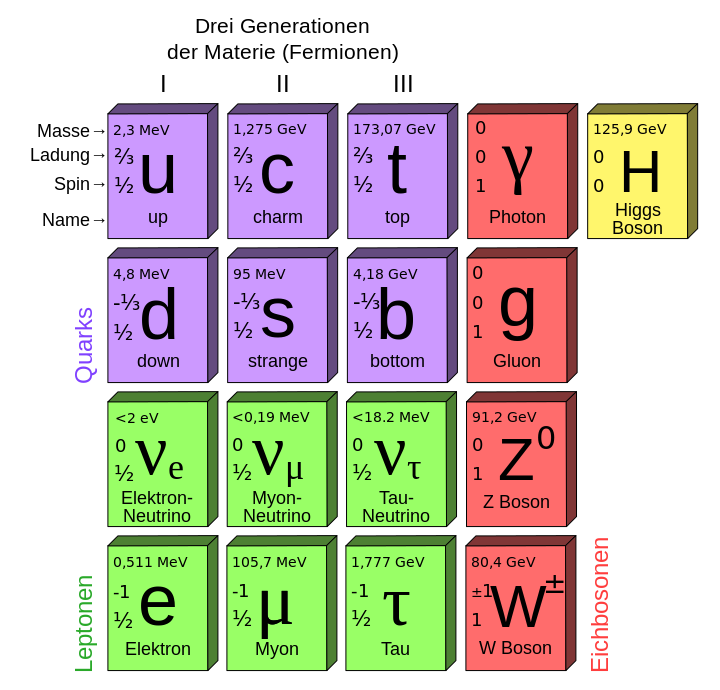
\includegraphics[width=\textwidth]{graphics/Standard_Model.png}
   \parbox[b]{12cm}{
     \caption[Standardmodell der Teilchenphysik]
             {\label{fig:Standardmodell} \it\!Die 12 fundamentalen Fermionen und 5 fundamentalen Bosonen des Standardmodells der Teilchenphysik,\\ Quelle: \cite{wiki:Standardmodell}}
   }
 \end{center}
\end{figure}

Insgesamt stimmen die experimentellen Ergebnisse gut mit den Vorhersagen des Standardmodells \"uberein. Dennoch reicht das Modell nicht aus, um s\"amtliche Ph\"anomene zu erkl\"aren. Im Modell werden beispielsweise masselose Neutrinos gefordert, allerdings wird zur Erkl\"arung der beobachteten Neutrinooszillationen die Existenz massiver Neutrinos ben\"otigt.

%% ===========================
\section{Assoziierte Higgs-Boson-Top-Quark-Paar-Produktion (\ttH)}
\label{ch:Theorie:sec:ttH}
%% ===========================

Da die Kopplungskonstante des Higgs-Mechanismus im Standardmodell von der Fermionenmasse abh\"angt, ist eine Untersuchung der Kopplung zwischen Top-Quark und Higgs-Boson aufgrund der hohen Masse des Top-Quarks verglichen mit anderen Quarkmassen, besonders interessant. In Tabelle \ref{tab:quarkmasse} sind zum Vergleich die Quarkmassen aufgelistet.\\


\begin{table}[hhh]\parbox{12cm}{
  \caption[Quarkmassen]{\it\!Tabelle mit Quarkmassen {\rm \cite{Agashe:2014kda}}
  }\label{tab:quarkmasse}}
  \begin{center}
  \begin{tabular}{lll}
  \hline
  {\bf Quark} & {\bf Symbol} & {\bf Masse}  \\
  \hline \hline
     Up		& u & $\num{2,3}^{{+0,7}}_{{-0,5}}\si{\mega\electronvolt}$ \\
     Down	& d & $\num{4,8}^{{+0,5}}_{{-0,3}}\si{\mega\electronvolt}$ \\
     Strange& s & $\num{95}\pm \num{5}\si{\mega\electronvolt}$ \\
     Charm	& c & $\num{1,275}\pm \num{0,025}\si{\giga\electronvolt}$ \\ 
  	 Bottom & b & $\num{4,18}\pm \num{0,03}\si{\giga\electronvolt}$ \\
     Top    & t & $\num{173,07}\pm \num{0,52}\pm \num{0,72}\si{\giga\electronvolt}$ \\                                   
  \hline
  \end{tabular}
  \end{center}
\end{table}

Diese Kopplung kann w\"ahrend der assoziierten Produktion eines Higgs-Bosons mit einem Paar aus Top-Quark und Anti-Top-Quark untersucht werden.\\
Wechselwirkungen zwischen Teilchen k\"onnen durch Feynman-Diagramme visualisiert werden. In Abbildung \ref{fig:ttH_feynmans} sind exemplarisch einige Feynmandiagramme zur \ttH-Produktion in f\"uhrender Ordnung abgebildet und zum Vergleich das Feynmandiagramm der Gluon-Gluon-Fusion, dem dominierenden Kanal der Higgs-Boson-Produktion am LHC, in Abbildung \ref{fig:gluonfusion}.

\begin{figure}[hhh]
 \begin{center}
   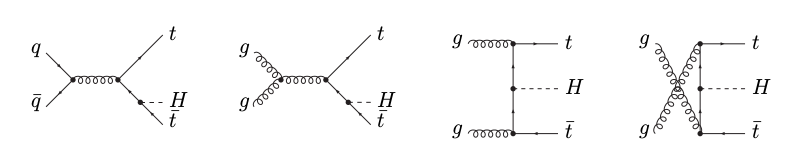
\includegraphics[width=\textwidth]{graphics/ttH_feynmans.png}
   \parbox[b]{12cm}{
     \caption[\ttH Feynman-Diagramme]
             {\label{fig:ttH_feynmans} \it\!Feynman-Diagramme f\"ur die \ttH-Produktion aus Hadronenkollisionen in f\"uhrender Ordnung \cite{hep-ph/0211352}}
   }
 \end{center}
\end{figure}

\begin{figure}[hhh]
 \begin{center}
   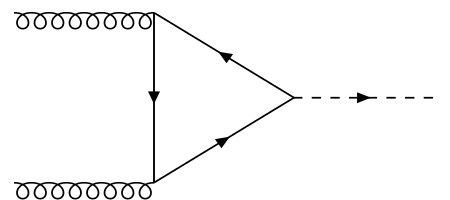
\includegraphics[width=0.4\textwidth]{graphics/gluonfusion.png}
   \parbox[b]{12cm}{
     \caption[Gluon-Gluon-Fusion Feynman-Diagramm]
             {\label{fig:gluonfusion} \it\!Feynman-Diagramm f\"ur die Gluon-Gluon-Fusion, dem dominierenden Kanal der Higgs-Boson-Produktion am LHC, erstellt mit \cite{feynman_draw}}
   }
 \end{center}
\end{figure}
%% Theorie.tex
%%
%\usepackage[ngerman]{babel}
%% ==============
\chapter{Experimentelle Grundlagen}
\label{ch:experiment}
%% ==============

%{\bibliographystyle{babalpha-fl}}	% german style
{\bibliographystyle{babunsrt-fl}}

Zur Untersuchung der theoretischen Vorhersagen des Standardmodells werden weltweit Experimente durchgef\"uhrt. In diesem Kapitel werden die experimentellen Grundlagen anhand des Compact-Muon-Solenoid-Experiment (CMS) vorgestellt. In Abschnitt \ref{ch:Experiment:sec:LHC} wird n\"aher auf den Large-Hadron-Collider (LHC), den gro\ss en Teilchenbeschleuniger des CERN eingegangen. Das CMS-Experiment wird in Abschnitt \ref{ch:Experiment:sec:CMS} genauer beschrieben.\\%(CMS, Abschnitt \ref{ch:Experiment:sec:CMS}) am Large-Hadron-Collider (LHC, Abschnitt \ref{ch:Experiment:sec:LHC}) des CERN vorgestellt. 
Anschlie\ss end wird der Ablauf einer Hochenergiephysik-Analyse am Beispiel der \ttH-Analyse vorgestellt.

%% ===========================
\section{Der Large Hadron Collider (LHC)}
\label{ch:Experiment:sec:LHC}
%% ===========================

Der Large-Hadron-Collider (LHC) ist ein Teilchenbeschleuniger der Europ\"aischen Organisation f\"ur Kernforschung (CERN). Er befindet sich in einem \num{26,7} Kilometer langen Tunnel im Grenzgebiet zwischen Frankreich und der Schweiz bei Genf zwischen \num{45} Meter und \num{170} Meter unter der Erdoberfl\"ache. Er ist der zur Zeit (\num{2016}) leistungsst\"arkste Teilchenbeschleuniger der Welt.\\
Der LHC kann mit Protonen oder Bleiionen betrieben werden. Wenn Protonen genutzt werden, durchlaufen diese zun\"achst eine Reihe von Vorbeschleunigern in denen sie pr\"apariert werden. Als erstes wird Wasserstoffgas ionisiert. Die so entstehenden Protonen werden im LINAC2, einem Linearbeschleuniger in B\"undeln (bunches) mit je $\num{1,1}\cdot\num{10}^{\num{11}}$ Protonen auf 50 MeV beschleunigt \cite{O'Luanaigh:1997427}. Anschlie\ss end werden die Protonenbunches im Proton-Synchrotron-Booster (PSB), im Proton-Synchroton (PS) und im Super-Proton-Synchrotron (SPS) erst auf 1,4 GeV, dann auf 25 GeV und schlie\ss lich auf 450 GeV beschleunigt \cite{O'Luanaigh:1997193}. Im LHC selbst werden in zwei Strahlr\"ohren jeweils maximal 2808 bunches in entgegengesetzte Richtungen auf maximal 7 TeV beschleunigt \cite{Lefevre:1165534}. Die Protonen werden an bestimmten Punkten zur Kollision gebracht. \\
Es gibt sieben Experimente, die die bei den Kollisionen entstehenden Teilchen untersuchen. Diese Experimente werden von Kollaborationen von Wissenschaftlern aus aller Welt durchgef\"uhrt. Die beiden gr\"o\ss ten sind ATLAS \cite{ATLAS} und CMS \cite{CMS}, die mit ihren universellen Teilchendetektoren alle entstehenden Kollisionsprodukte au\ss er Neutrinos untersuchen k\"onnen, w\"ahrend bei dem Schwerionen-Experiment ALICE (A Large Ion Collider Experiment) und dem Large-Hadron-Collider-beauty-Experiment (LHC-B) spezifische Ph\"anomene untersucht werden. ALICE wurde entwickelt um durch Kollisionen von Bleiionen ein Quark-Gluon-Plasma zu erzeugen, was den Bedingungen kurz nach dem Urknall entspricht \cite{ALICE}. LHC-B untersucht Unterschiede zwischen Materie und Antimaterie mithilfe von b-Quarks \cite{LHCb}. Die kleineren Experimente sind TOTEM (Total, elastic and diffractive cross-section measurement) und LHCf (Large Hadron Collider forward), die beide in Richtung des Strahls (\glqq vorw\"arts\grqq) gestreute Ereignisse, also Ereignisse mit sehr kleinem Streuwinkel untersuchen \cite{LHCf,TOTEM} sowie MoEDAL (Monopole and Exotics Detector at the LHC), das nach magnetischen Monopolen sucht \cite{MoEDAL}.\\%\cite{O'Luanaigh:1997374, O'Luanaigh:1997265, O'Luanaigh:1997262, O'Luanaigh:1997259, O'Luanaigh:1997373, O'Luanaigh:1997527}.\\
In Abbildung \ref{fig:LHC} ist der schematische Aufbau des LHC mit den Experimenten CMS, ATLAS, LHC-B und ALICE abgebildet. Die Vorbeschleuniger sind dabei bis auf das Super-Proton-Synchrotron nicht ber\"ucksichtigt.

\begin{figure}[hhh]
 \begin{center}
   \includegraphics[width=0.8\textwidth]{graphics/LHC_experiments.jpg}
   \parbox[b]{12cm}{
     \caption[Large-Hadron-Collider]
             {\label{fig:LHC} \it\!Der LHC mit den vier Hauptexperimenten und dem Super-Proton-Synchrotron \cite{Team:40525}}
   }
 \end{center}
\end{figure}

%% ===========================
\section{Der Compact-Muon-Solenoid-Detektor (CMS)}
\label{ch:Experiment:sec:CMS}
%% ===========================

Der Compact-Muon-Solenoid (CMS) ist einer der beiden universellen Teilchendetektoren am LHC. Sein Aufbau ist in Abbildung \ref{fig:cms_sectional} zu sehen. Der Detektor ist etwa \num{14000} Tonnen schwer und hat einen Durchmesser von \num{15} Metern bei einer L\"ange von \num{28,7} Metern. Die einzelnen Teile des Detektors wurden \"uberirdisch gefertigt und in einer Kaverne in ungef\"ahr \num{100} Metern Tiefe zusammengebaut.
\begin{figure}[hhh]
 \begin{center}
   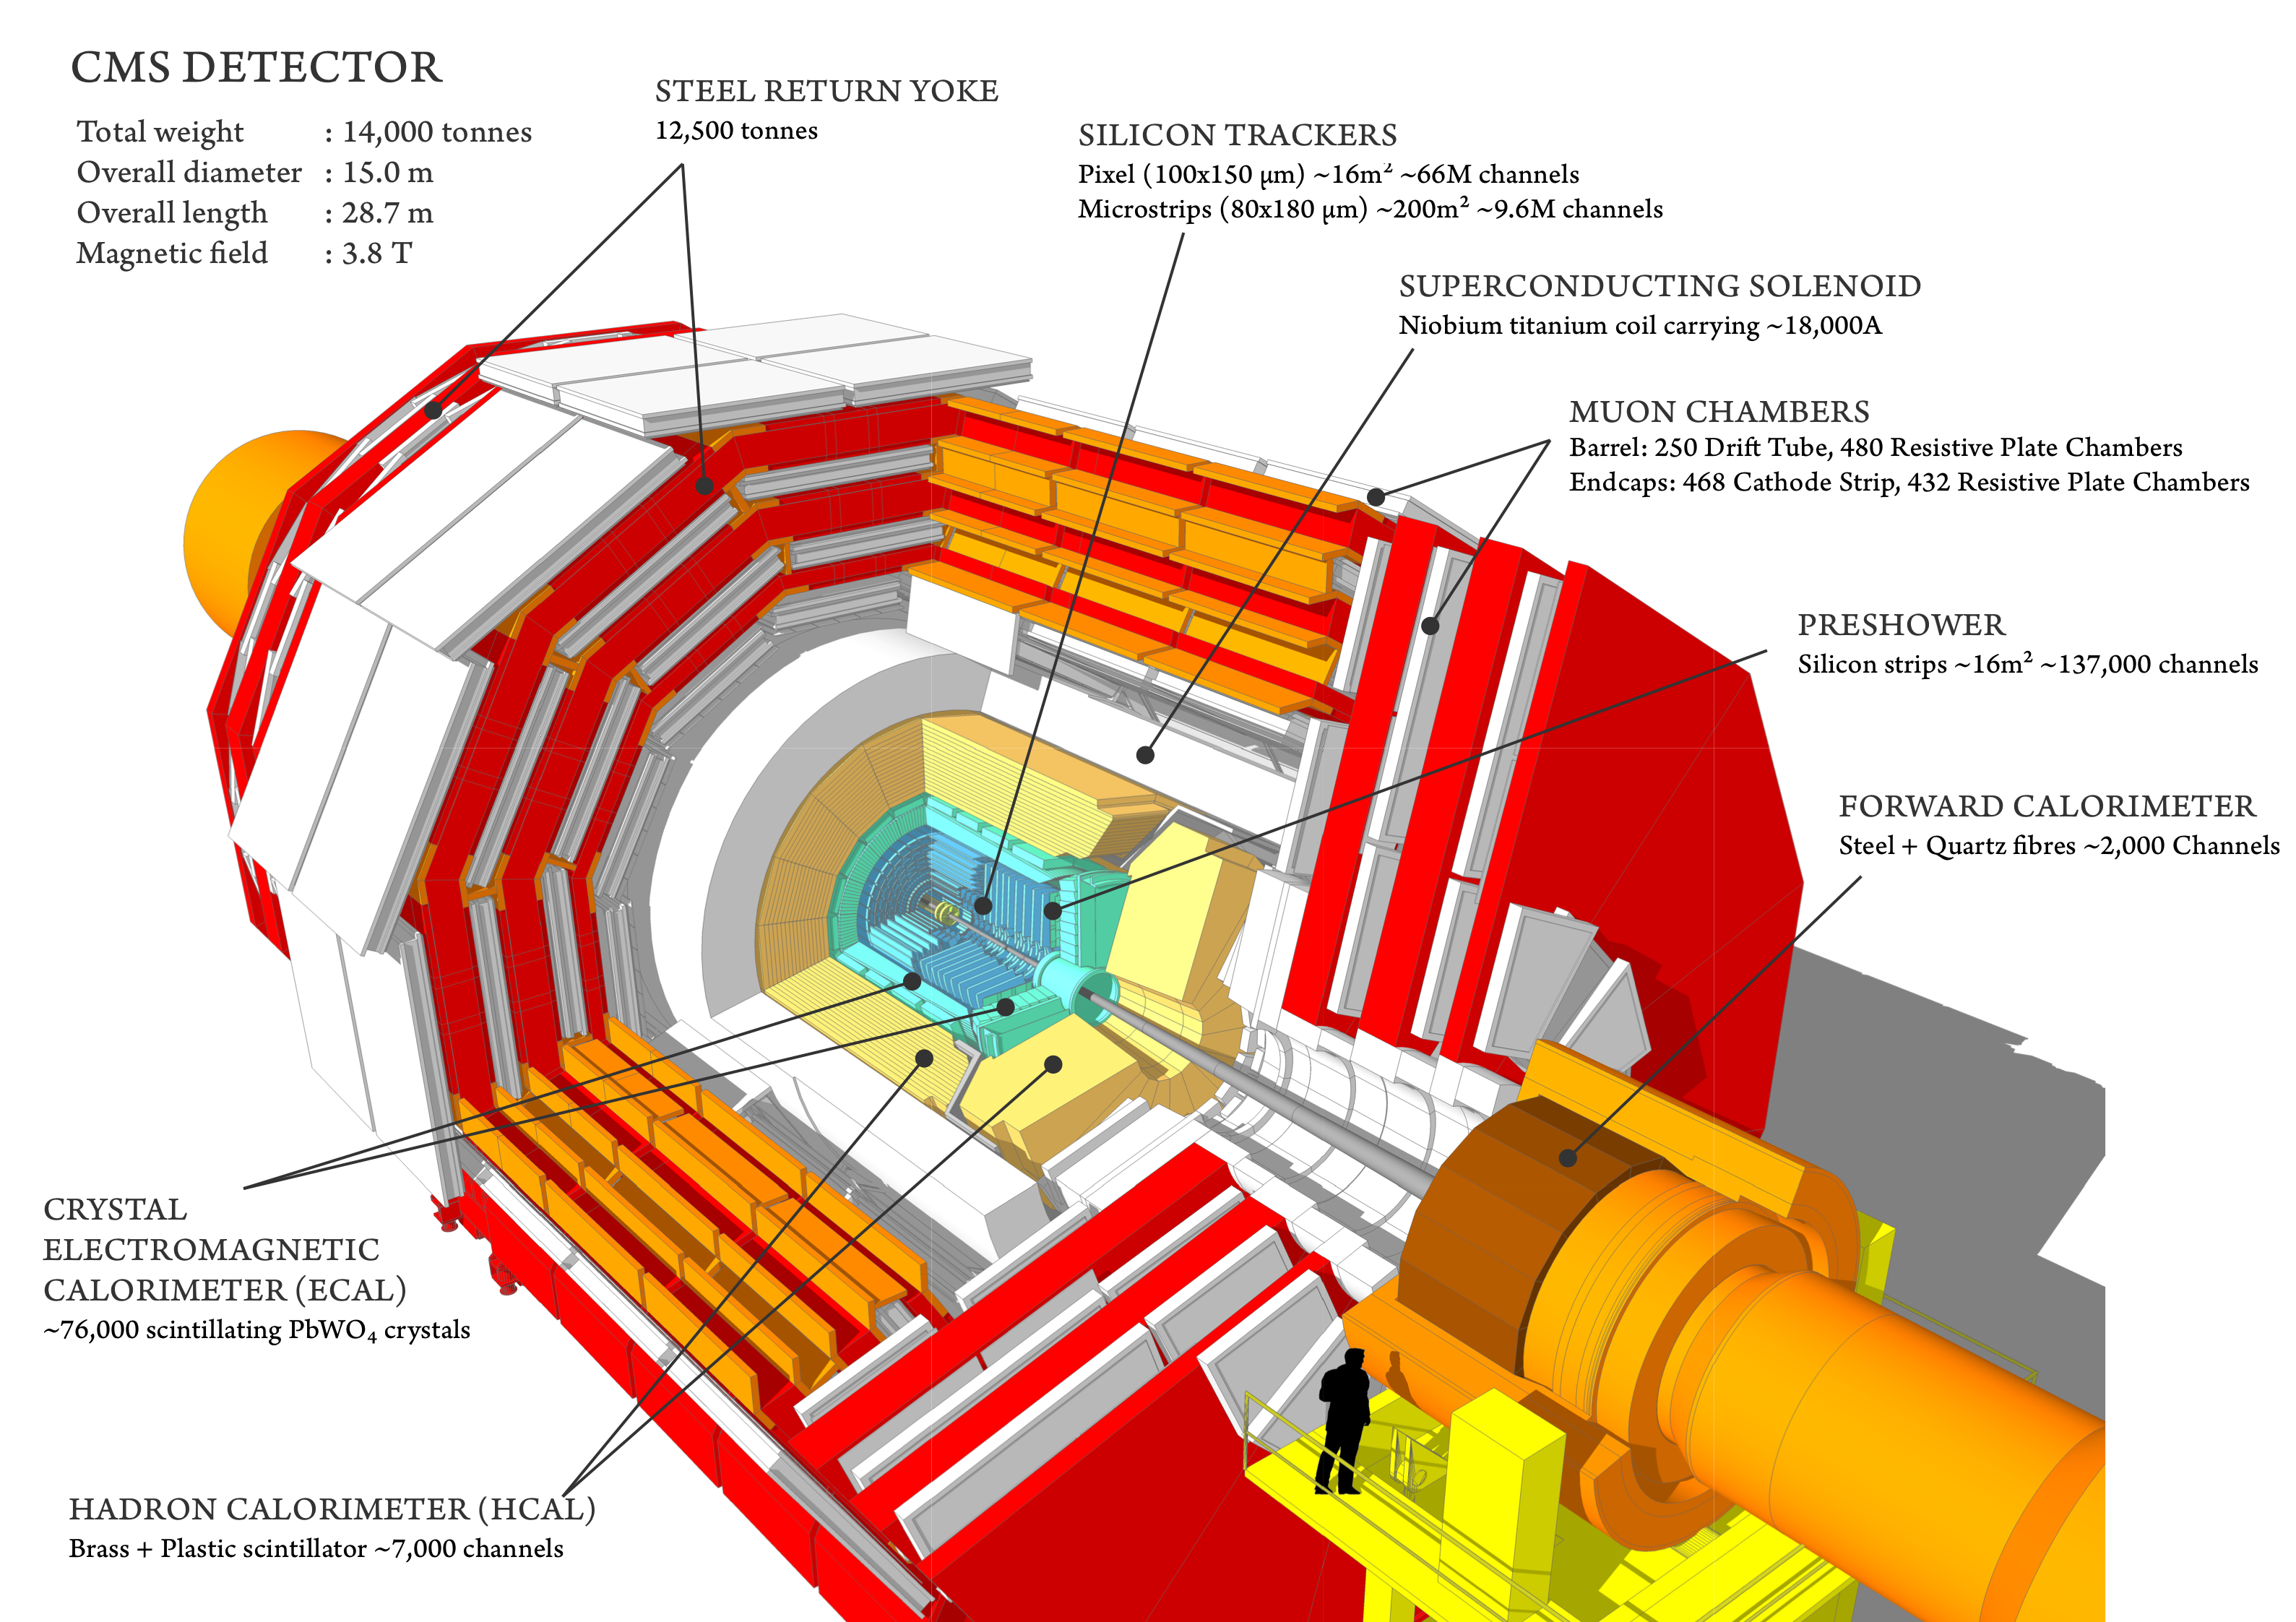
\includegraphics[width=\textwidth]{graphics/cms_sectional.png}
   \parbox[b]{12cm}{
     \caption[CMS-Detektor]
             {\label{fig:cms_sectional} \it\!Der CMS-Detektor im Querschnitt \cite{cms_sectional}}
   }
 \end{center}
\end{figure}

Das CMS-Experiment besteht aus mehreren Detektoren, die in zylinderf\"ormigen Lagen, \"ahnlich einer Zwiebel, \"ubereinandergeschichtet sind. Namensgebendes St\"uck ist der gro\ss e Magnet (solenoid), der ein bis zu \num{4} Tesla starkes homogenes Magnetfeld erzeugen kann. Dadurch werden geladene Teilchen abgelenkt und ihr Impuls kann bestimmt werden. Die innerste Lage des CMS bildet der Spurdetektor. Er besteht aus Silizium-Pixeldetektoren und Silizium-Streifendetektoren. Sie bestimmen die Spuren der bei der Kollision erzeugten Teilchen. Als n\"achste Schicht ist ein elektromagnetisches Kalorimeter (ECAL) aus Bleiwolframat-Kristallen (PbWO$_4$) eingebaut. Damit k\"onnen Elektronen, Positronen und Photonen nachgewiesen und ihre Energie bestimmt werden. Das ECAL wird umschlossen von einem hadronischen Kalorimeter (HCAL), das zur Identifizierung und Energiemessung der Hadronen verwendet wird. An diese Lage schlie\ss t sich die Magnetspule an. Au\ss erhalb des Magneten befinden sich das eiserne R\"uckf\"uhrjoch, das von Myonenkammern zum Nachweis von Myonen durchzogen ist.\\

\begin{figure}[hhh]
 \begin{center}
   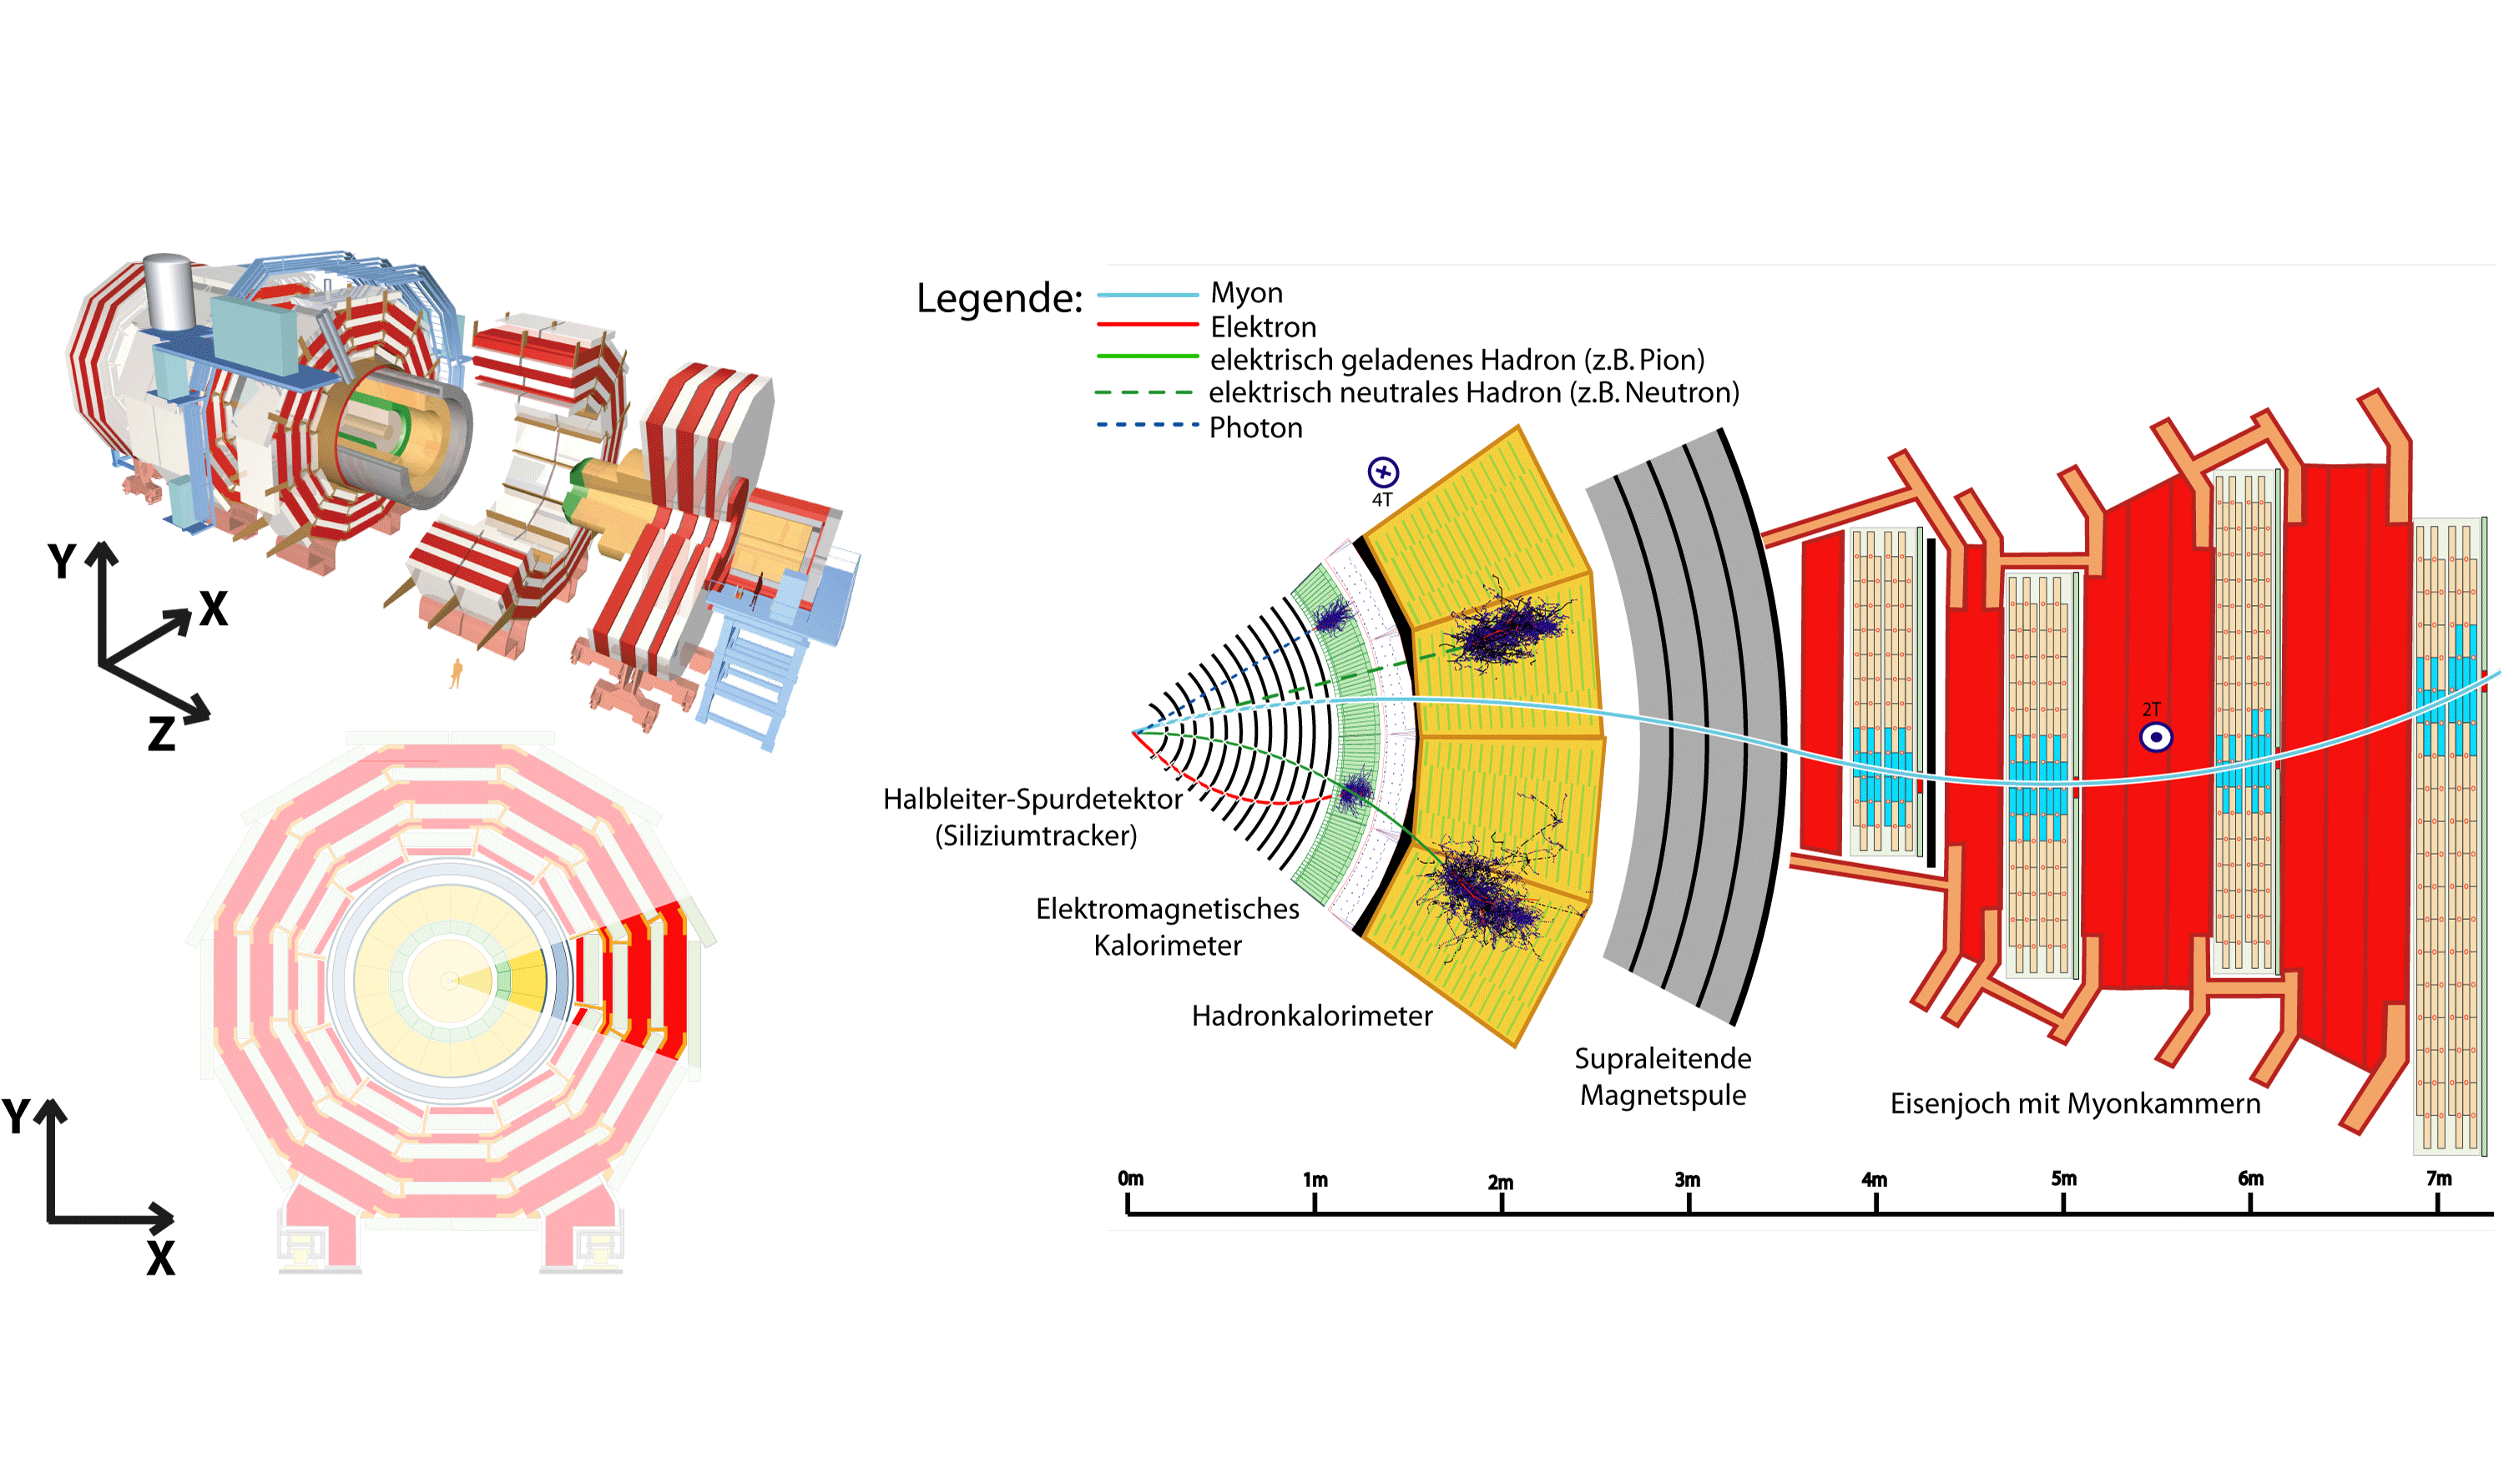
\includegraphics[width=\textwidth]{graphics/cms_slice.png}
   \parbox[b]{12cm}{
     \caption[CMS-Detektor]
             {\label{fig:cms_slice} \it\!Ausschnitt des CMS-Detektors mit verschiedenen Teilchenbahnen \cite{cms_slice}}
   }
 \end{center}
\end{figure}

In Abbildung \ref{fig:cms_slice} ist nochmals ein Ausschnitt des CMS-Detektors mit den Trajektorien der einzelnen Teilchen abgebildet. Im linken oberen Bereich ist der komplette Detektor mit auseinandergefahrenen Segmenten zu sehen. Darunter ist der Querschnitt gezeigt, die hervorgehobene Sektion ist rechts daneben gr\"o\ss er dargestellt. Man erkennt die einzelnen Schichten des Detektors. Die rote Linie zeigt beispielhaft das Verhalten eines Elektrons, das w\"ahrend es den Spurdetektor durchl\"auft vom Magnetfeld abgelenkt wird und schlie\ss lich im elektromagnetischen Kalorimeter einen Schauer erzeugt wodurch es detektiert werden kann. In gr\"un sind die Trajektorien von Hadronen gezeigt. Die gestrichelte Linie entspricht einem ungeladen, die durchgezogene einem positiv geladenen. Beide erzeugen im Hadronenkalorimeter Schauer. Wie ein ungeladenes Hadron wird auch ein Photon (blau gestrichelte Linie) nicht vom Magnetfeld abgelenkt, allerdings erzeugt es bereits im ECAL einen Schauer. Ein Anti-Myon (blaue durchgezogene Linie) wird erst in den Myonenkammern detektiert. %interagiert nicht mit den inneren Schichten des Detektors und wird daher erst in den Myonenkammern detektiert.

%% ===========================
\section{\ttH-Analyse}
\label{ch:Experiment:sec:ttH}
%% ===========================

Der Wirkungsquerschnitt der \ttH-Produktion ist klein und es gibt viele andere Prozesse, die zum Untergrund beitragen. Deshalb ist es anspruchsvoll, die Produktionsrate zu messen. Im Folgenden soll die \ttH-Analyse am CMS-Experiment kurz erl\"autert werden. Einige der verwendeten und dar\"uberhinausf\"uhrende Informationen finden sich in \cite{Khachatryan:2014qaa}.

Der \ttH-Analyse liegen durch das Standardmodell motivierte Berechnungen zugrunde. Anhand der verschiedenen vorhergesagten Endzust\"ande werden die einzelnen Produktionskan\"ale in verschiedene Kategorien unterteilt, die sich in wesentlichen Punkten unterscheiden. Mithilfe von Teilchenphysikalischen Methoden, wie dem Erkennen von Bottom-Quarks (b-tagging), auf die hier nicht n\"aher eingegangen wird, werden f\"ur die verschiedenen Kollisionsprodukte physikalische Eigenschaften bestimmt. Diese k\"onnen beispielsweise Transversalimpuls oder rekonstruierte teilchenmasse sein, aber teilweise auch Kombinationen von Eigenschaften mehrerer rekonstruierter Teilchen, etwa Winkelverteilungen zwischen den Teilchen. Da die meisten bei Proton-Proton-Kollisionen produzierten Ereignisse keine \ttH-Ereignisse sind, m\"ussen sie von den viel h\"aufigeren Untergrundereignissen unterschieden werden. Hierf\"ur werden multivariate Analysemethoden (MVA-Methoden) verwendet, welche die oben genannten Eigenschaften kombinieren.\\
%Um die gesuchten Ereignisse aus den anderen Produkten der Teilchenkollissionen herauszufiltern, werden Multivariate Analysemethoden (Kapitel \ref{ch:algorithmen}) verwendet.\\
Dazu ist es entscheident die Struktur der aufgenommenen Daten bereits zu kennen. Aus diesem Grund werden mithilfe von Monte-Carlo-Methoden, die auf theoretische Berechnungen sowie Wissen \"uber das Detektorverhalten basieren, Simulationsdaten erstellt. Die gew\"unschten und gesuchten Ereignisse sind in den Simulationsdaten daher ebenso wie die unerw\"unschten Untergrunddaten bekannt.\\% Auf die simulierten Daten werden nun multivariate Algorithmen angewandt, die anhand der konstruierten Eigenschaften erlernen die Signal- von den Untergrundereignissen zu unterscheiden. Dadurch lernen die Algorithmen selbst\"andig (machine learning) verschiedenartige Daten zu unterscheiden.\\ %Damit wird versucht aus den experimentell gemessenen Daten die gesuchten \ttH-Ereignisse zu extrahieren.\\
Auf die simulierten Daten werden nun multivariate Algorithmen angewendet. Die Algorithmen erlernen dabei anhand der Ereigniseigenschaften die Unterscheidung von Signal und Untergrund. Aufgrund dieses Lernprozesses bezeichnet man dies auch als machine learning.\\
Zuletzt werden die trainierten Algorithmen auf die im echten Detektor gemessenen Daten angewandt. Die somit erhaltenen Ergebnisse werden dann mit den simulierten Daten verglichen und die \"Ubereinstimmung mit der Vorhersage des Standardmodells gepr\"uft.

%% Theorie.tex
%%
%\usepackage[ngerman]{babel}
%% ==============
\chapter{Algorithmen zur multivariaten Analyse}
\label{ch:algorithmen}
%% ==============

%{\bibliographystyle{babalpha-fl}}	% german style
{\bibliographystyle{babunsrt-fl}}

Multivariate Datenanalyse spielt in der experimentellen Teilchenphysik eine entscheidente Rolle, um die gro\ss en gemessenen Datenmengen untersuchen und auswerten zu k\"onnen. In diesem Kapitel werden zun\"achst einige Grundlagen der multivariaten Datenanalyse genannt, um sp\"ater genauer auf verschiedene Algorithmen und ihre Implementierungen einzugehen.

%% ===========================
\section{Grundlagen zur multivariaten Datenanalyse}
\label{ch:Theorie:sec:Algorithmen}
%% ===========================

Datenanalyse bezeichnet statistische Verfahren, mit deren Hilfe aus numerischen Daten Informationen gewonnen werden.
Bei multivariaten Analysemethoden (MVAs) werden mehrere Eingabegr\"o\ss en gleichzeitig statistisch untersucht. Dadurch ist eine Berechnung sehr aufw\"andig und somit manuell praktisch nicht zu bewerkstelligen. Mithilfe der zunehmenden Rechenleistung aktueller Computer ist dies jedoch m\"oglich und wird in vielen Bereichen immer wichtiger. Anwendungen finden MVAs beispielsweise im Finanzwesen, oder der Sprach-, Schrift- und Bilderkennung.\\
%Da die verwendeten Algorithmen die Eigenschaft haben anhand von bekannten Daten Vorhersagen f\"ur unbekannte Daten zu generieren, spricht man auch von maschinellem Lernen (machine learning).
%Die dazu verwendeten Algorithmen bezeichnet man auch als maschinelles Lernen (machine learning), da mit ihrer Hilfe versucht wird, die zugrunde liegenden Eigenschaften der Daten zu Lernen und Vorhersagen zu treffen.
Ziel ist es, mithilfe der Algorithmen aus bekannten Daten zu lernen und so Vorhersagen f\"ur unbekannte Daten zu generieren.
Man unterscheidet zwischen Regression, bei der eine kontinuierliche Ausgangsgr\"o\ss e gesucht wird, und Klassifikation, bei der eine diskrete Antwort gesucht wird \cite{SWB-455193959}.

Im Fall der \ttH-Analyse werden Regressionsmodelle verwendet, um physikalische Gr\"o\ss en wie beispielsweise die Higgs-Bosonmasse zu rekonstruieren. Bei der Klassifikation wird dagegen versucht, ein Ereignis einer Klasse zuzuordnen, also entweder Signal oder Untergrund. Im Folgenden werden ausschlie\ss lich Klassifikationsprobleme behandelt.

Die St\"utzvektormethode (support vector machine), Random Forest und Neuronale Netze sind Beispiele f\"ur Methoden zur Klassifikation. 
%Es existieren verschiedene Ans\"atze zur Klassifikation. Beispiele sind die St\"utzvektormethode, wobei jedoch die englische Bezeichnung support vector machine (SVM) gebr\"auchlich ist, Random Forest (RF), was zuf\"alliger Wald bedeutet und mehrere zuf\"allig erstellte Entscheidungsb\"aume (Abschnitt \ref{ch:Algorithmen:subsec:Entscheidungsbaum}) bezeichnet, oder Neuronale Netze. 
Ein weiteres Beispiel sind verst\"arkte Entscheidungsb\"aume (Boosted Decision Trees (BDTs)). Da hiervon verschiedene Implementationen im Kapitel \ref{ch:vergleich} untersucht und getestet werden sollen, werden sie im folgenden Abschnitt \ref{ch:Algorithmen:sec:BDT} genauer beschrieben.

%% ===========================
\section{Verst\"arkte Entscheidungsb\"aume}
\label{ch:Algorithmen:sec:BDT}
%% ===========================

Verst\"arkte Entscheidungsb\"aume (Boosted Decision Trees, BDTs) sind eine h\"aufig genutze Methode der multivariaten Datenanalyse. Im Folgenden werden sie anhand eines Beispiels erkl\"art. Bei diesem handelt es sich um zwei zweidimensionale Gau\ss verteilungen die sich \"uberlappen. Eine stellt das Signal dar, die andere dient als Untergrund. Der Erwartungswert der Signalverteilung ist bei $\mu_X=\mu_Y=0$, der der Untergrundverteilung bei $\mu_X=\mu_Y=1$. Beide haben eine Standardabweichung von $\sigma=1$. In Abbildung \ref{fig:2dgauss_scat} ist ein Streudiagramm mit Trainings-Datenpunkten dargestellt. Insgesamt haben sowohl Signal als auch Untergrund 10001 Ereignisse, zur besseren \"Ubersicht sind allerdings nur jeweils 1000 dargestellt.\\
Die folgenden Abschnitte sind gr\"o\ss tenteils an \cite{SWB-307748006} angelehnt.

\begin{figure}[tbp]
 \begin{center}
   \includegraphics[width=\textwidth]{graphics/2d_scatter.pdf}
   \parbox[b]{12cm}{
     \caption[Streudiagramm mit Trainings-Datenpunkten]
             {\label{fig:2dgauss_scat}Ein Streudiagramm mit je 1000 Signal- und Untergrundereignissen. Signalereignisse sind rot, Untergrundereignisse blau dargestellt.}
   }
 \end{center}
\end{figure}

%% ===========================
\subsection{Entscheidungsb\"aume}
\label{ch:Algorithmen:subsec:Entscheidungsbaum}
%% ===========================

Entscheidungsb\"aume (Decision Trees) unterteilen den Bereich der zu klassifizierenden Objekte anhand gerader Schnitte auf dessen Eigenschaften (Variablen) in mehrere Sequenzen. Wieviele dieser Sequenzen ab dem Wurzelknoten erstellt werden, wird durch die Tiefe (depth) des Baumes angegeben. Man unterscheidet zwischen zwei Arten, bin\"aren B\"aumen mit diskreten R\"uckgabewerten zur Unterscheidung mehrerer Klassen (classification trees), zum Beispiel Signal und Untergrund sowie denjenigen mit kontinuierlicher Antwort (regression trees) \cite{SWB-455193959}. Eine h\"aufige Implementierung von Entscheidungsb\"aumen ist CART (classification and regression trees). Auf diese Weise implementierte B\"aume eignen sich sowohl f\"ur Klassifikationen als auch f\"ur Regressionen \cite{CART}.\\
In Abbildung \ref{fig:DecicionTree} ist ein Beispiel eines Baumes mit der Tiefe zwei zu sehen. An jedem Knoten werden die Objekte aufgrund ihrer Eigenschaften und Kriterien in Signal und Untergrund unterteilt. Im Wurzelknoten ist der erste diskriminierende Schnitt angegeben. Alle Objekte mit einem Y-Wert gr\"o\ss er als \num{0,4} werden als untergrundartig eingestuft. In der n\"achsten Stufe des Baumes werden f\"ur jede der beiden zuvor getrennten Mengen Schnitte auf den X-Wert angewendet. In Abbildung \ref{fig:depht2} ist die Ausgabe (output) dieses Baumes abgebildet. Das hei\ss t, jedem Punkt wird entsprechend seiner X- und Y-Koordinaten ein Wert zugeordnet, der angibt, ob der Punkt eher als Signal oder als Untergrund klassifiziert wurde. H\"ohere Werte werden f\"ur signalartige Punkte verwendet, niedrigere f\"ur untergrundartige. Es sind die verschiedenen Schnitte des Baumes zu erkennen.\\
%\begin{figure}[tbp]
% \begin{center}
%  \begin{minipage}[b]{0.5\textwidth}  
%   \includegraphics[width=\textwidth]{graphics/tree.pdf}
%   \centering (a)
%  \end{minipage}%
%  \begin{minipage}[b]{0.5\textwidth}
%   \includegraphics[width=\textwidth]{graphics/tree_depht2.pdf}
%   \centering (b)
%  \end{minipage}
%   \parbox[b]{12cm}{
%     \caption[Entscheidungsbaumes der Tiefe 2]
%             {\label{fig:DecicionTree} \it schematische Abbildung eines Entscheidungsbaumes der Tiefe 2. X und Y sind die Variablen anhand denen durch cuts (Zahlen nach den Variablen) zwischen Untergrund und Signal unterschieden werden soll.\\Erstellt mit TMVA}
%   }
% \end{center}
%\end{figure}

\begin{figure}[tbp]
\centering     %%% not \center
\subfigure[Entscheidungsbaum der Tiefe zwei]{\label{fig:DecicionTree}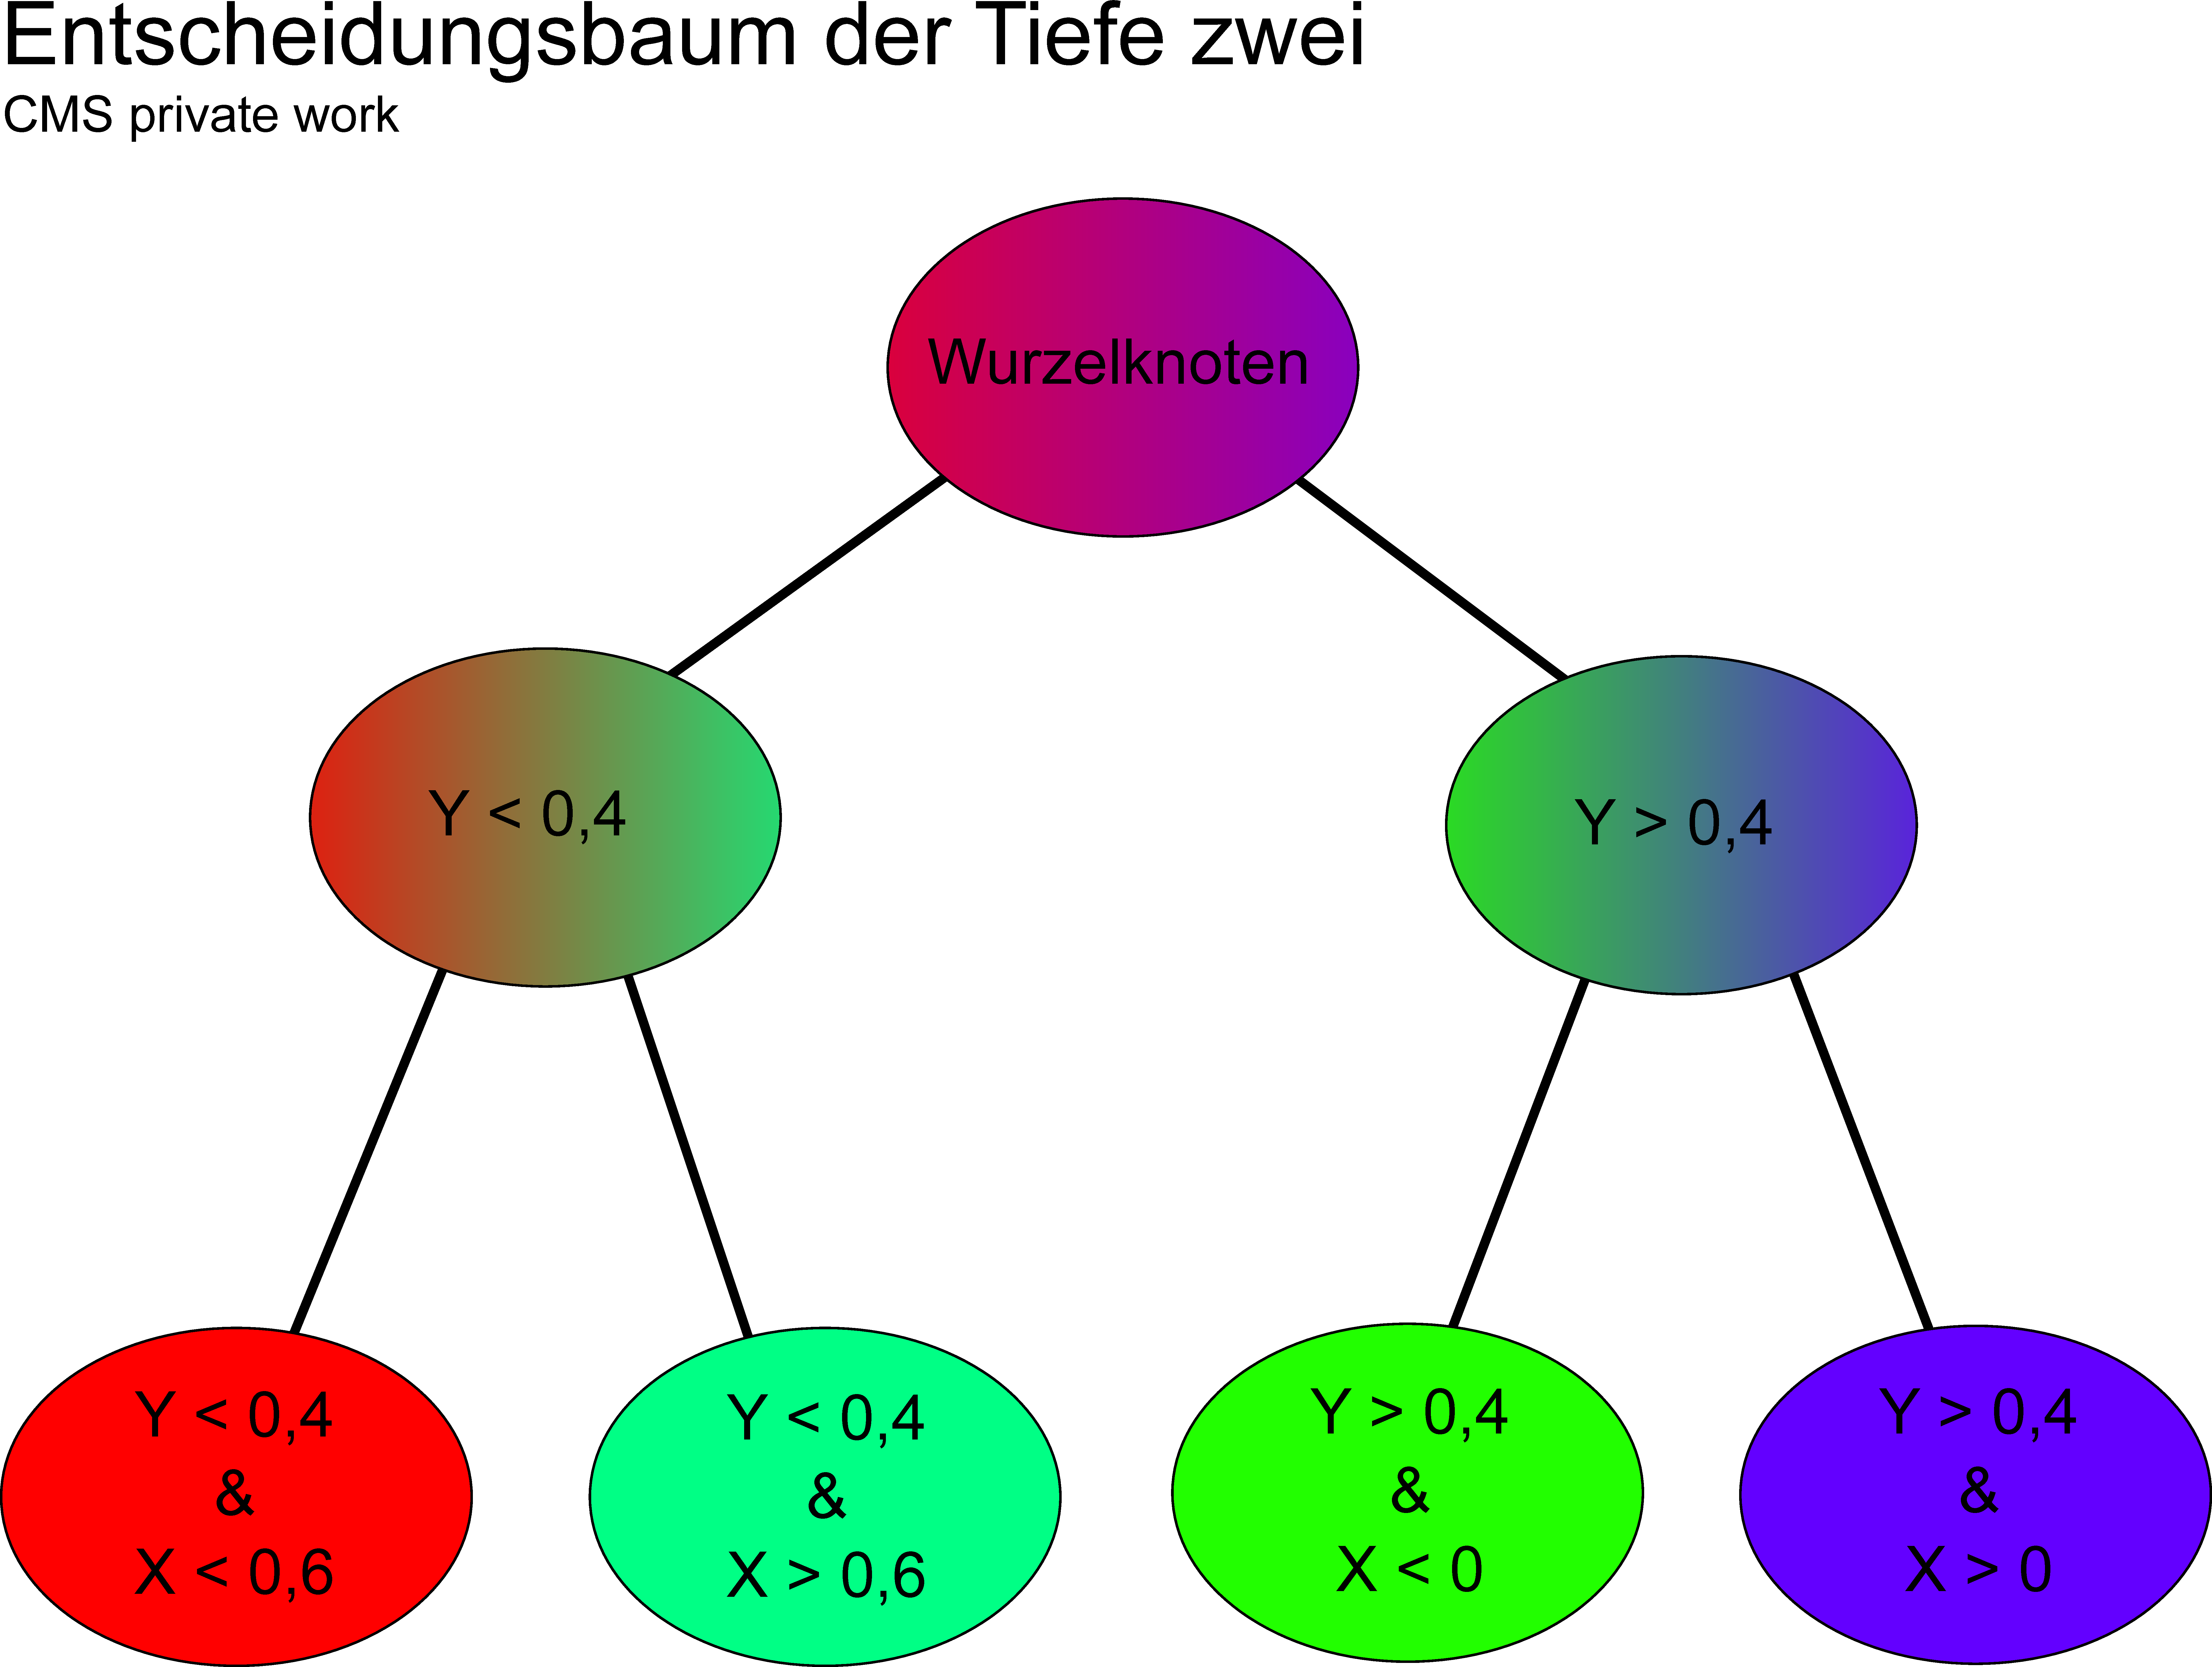
\includegraphics[width=0.7\textwidth]{graphics/tree_d22.pdf}}
\subfigure[Klassifizierung des Baumes]{\label{fig:depht2}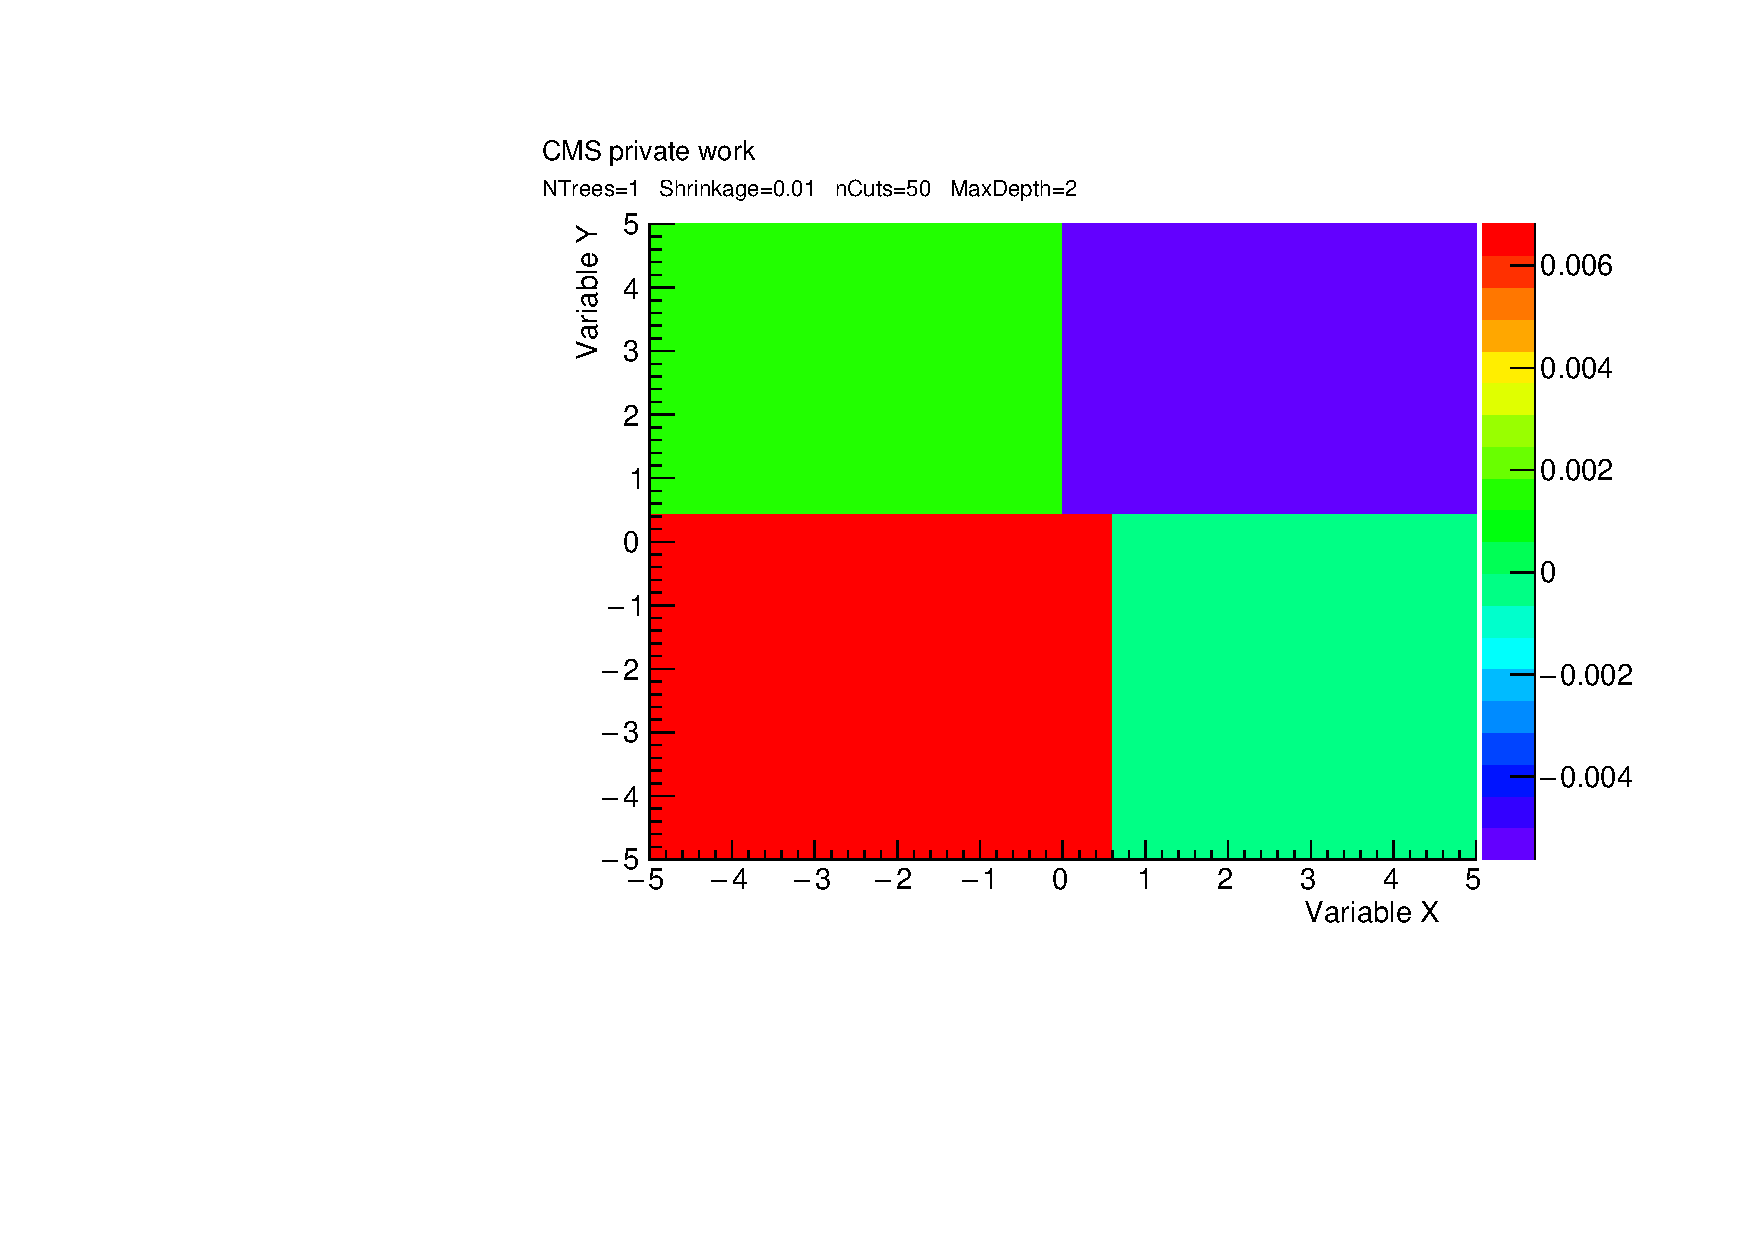
\includegraphics[width=0.85\textwidth]{graphics/tree_depht2_1.pdf}}
\parbox[b]{12cm}{
\caption{Oben ist eine schematische Abbildung eines Entscheidungsbaumes der Tiefe 2 abgebildet. X und Y sind die Variablen, anhand derer durch Schnitte (Zahlen nach den Variablen) zwischen Untergrund und Signal unterschieden werden soll. Die untere Graphik zeigt die Klassifikation, die mithilfe des Baumes erstellt wurde. Gr\"o\ss ere Ausgabewerte sind rot gef\"arbt und stehen f\"ur signalartige Ereignisse, kleinere blau und stehen f\"ur untergrundartige Ereignisse.}
}
\end{figure}

Die Trennung ist allerdings noch sehr grob, selbst wenn man die Tiefe des Baumes deutlich erh\"oht, wie in Abbildung \ref{fig:tree_depht100} mit der Tiefe 100 zu sehen, wird diese nicht deutlich besser. Eine Verbesserung ist beispielsweise m\"oglich, indem man mehrere Entscheidungsb\"aume so miteinander verkn\"upft, dass sie zusammen eine starke Klassifikation erm\"oglichen. Eine dieser Methoden ist das Verst\"arken von Entscheidungsb\"aumen (Boosting).




%BDTs vereinen durch Boosting und Bagging (aus dem Englischen von bootstrap aggregation abgeleitet) mehrere Entscheidungsb\"aume zu einem starken Kla\ss ifikator.

%% ===========================
\subsection{Verst\"arken von Entscheidungsb\"aumen}
\label{ch:Algorithmen:subsec:Boosting}
%% ===========================

Durch das Verst\"arken von Entscheidungsb\"aumen (Boosting) soll die G\"ute der Gesamtklassifikation gegen\"uber der eines einzelnen Baumes erh\"oht werden. Dazu werden mehrere B\"aume hintereinander trainiert. Damit diese sich voneinander unterscheiden, werden bei nachfolgenden B\"aumen die falsch klassifizierten Ereignisse anders behandelt\\
Die einfachste Methode ist, das Gewicht jedes falsch klassifizierten Ereignisses auf die gleiche Weise anzupassen. Eine weitere Verbesserung l\"asst sich erzielen, indem man eine Ausgleichsfunktion (loss function) einf\"uhrt. Diese ordnet jedem Ereignis ausgehend von der aktuellen BDT-Ausgabe einen Wert zu, der bei richtiger Klassifikation minimal ist. Dadurch ist es m\"oglich, die Gewichte so anzupassen, dass die Ausgleichsfunktion minimiert wird.\\
Wenn die zu trennenden Klassen mit $y=\pm1$ bezeichnet werden und $f(x)$ die Vorhersage des BDTs f\"ur das Ereignis $x$ ist, also $sign(f)$ die jeweilige Klasse vorhersagt, so kann man die einfache Methode der Neugewichtung mathematisch mit
\beq
L = I(sign(f(x))\neq y)
\label{eq:missclass_loss}
\eeq
beschreiben. Dabei nimmt die Funktion I den Wert $1$ an, wenn die Vorhersage nicht der wahren Klasse $y$ entspricht oder $0$, wenn die vorhergesagte mit der wahren Klasse \"ubereinstimmt.\\
Eine etwas komplexere Ausgleichsfunktion ber\"ucksichtigt die quadratischen Fehler der BDT-Vorhersage
\beq
L = (y-f(x))^2.
\label{eq:squarederror_loss}
\eeq
Diese Funktion bildet eine Parabel um den wahren Wert. Je weiter die Vorhersage davon abweicht, desto h\"oher wird das Ereignis gewichtet. Nachteilig ist dabei, dass positive wie negative Differenzen gleich stark korrigiert werden. So werden beispielsweise f\"ur $y=1$ BDT-Ausgaben von $f=0$ und $f=2$ gleich stark korrigiert, obwohl $f=0$ gar keine Klassifikation zul\"asst, w\"ahrend $f=2$ deutlich auf $y=1$ hinweist. Daher verwendet man meist Funktionen, die negative Abweichungen st\"arker umgewichten, wie beispielsweise die exponentielle Ausgleichsfunktion
\beq
L = \exp(-y\cdot f(x)).
\label{eq:exp_loss}
\eeq
Diese Ausgleichsfunktion wird beispielsweise von AdaBoost (kurz f\"ur Adaptive Boosting) \cite{ADABoost}, dem ersten entwickelten Boosting-Algorithmus, verwendet. Problematisch an der exponentiellen Ausgleichsfunktion ist, dass sie nicht besonders robust gegen\"uber Ausrei\ss ern ist.\\
Dieses Problem behebt der Gradient-Boosting-Algorithmus \cite{Friedman00greedyfunction}. Dabei wird eine zus\"atzliche Ausgleichsfunktion $L$ definiert, die nicht mithilfe der \"ublichen Vorgehensweise minimiert werden kann, sondern \"uber einen Ansatz der steilsten Abnahme (steepest-descent) minimiert werden muss. Dazu wird zun\"achst der negative Gradient der Ausgleichsfunktion gebildet:
\beq
r_m=\left|\frac{\partial L(y,f(x))}{\partial f(x)}\right|_{f=f_{m-1}}.
\label{eq:pseudo_residual}
\eeq
Die $r_m$ nennt man auch Pseudo-Residuen. Hierbei bezeichnet $m$ die jeweilige Boosting-Iteration. Danach wird ein zus\"atzlicher Regressionsbaum trainiert, f\"ur den als Zielwerte die Pseudo-Residuen anstatt der Klassen $y$ verwendet werden \cite{Hocker:2007ht}.\\
Die Endknoten des Regressionsbaums bezeichnet man mit $R_{jm}$, wobei $j$ den jeweiligen Knoten und $m$ den aktuellen Klassifikationsbaum numeriert. Insgesamt erh\"alt man eine BDT-Ausgabe von
\beq
\hat f(x) = f_M(x),
\eeq
wobei jede Iteration wie
\beq
f_m(x) = f_{m-1}+\nu\cdot\sum_{j=1}^J\gamma_{jm}I(x \in R_{jm})
\eeq
berechnet wird.\\
Dabei ist $\gamma_{jm}$ die Stelle, an der die Ausgleichsfunktion minimal wird. Die Funktion $I$ nimmt die Werte $1$ oder $0$ an, je nachdem ob das Ereignis $x$ im entsprechenden Endknoten des Regressionsbaumes liegt oder nicht. Die Gesamtanzahl der trainierten B\"aume ist $M$.
Der Parameter $\nu$ ist die Lernrate (shrinkage oder learning rate), der Werte von Null bis Eins annehmen kann. Mit diesem Parameter kann die Boosting Prozedur kontrolliert werden. Je kleiner der Wert ist, desto geringer werden die neu trainierten B\"aume gewichtet. Somit kann einem Erlernen von statistischen Fluktuationen entgegengewirkt werden (siehe auch Abschnitt \ref{ch:Algorithmen:subsec:overtraining}). Bei kleiner Lernrate sollte die Anzahl an B\"aumen h\"oher gew\"ahlt werden als bei gr\"o\ss erer. Die Bezeichnungen dieser und weiterer Optionen mit kurzer Erkl\"arung sind in Abschnitt \ref{ch:Vergleich:sec:Vergleichbarkeit} beschrieben.

In Abbildung \ref{fig:boosting} sind zum Vergleich die R\"uckgabewerte von einem einzelnen Entscheidungsbaum der Tiefe 100 (Abbildung \ref{fig:tree_depht100}) sowie diejenigen von BDTs der Tiefe zwei mit zwei (Abbildung \ref{fig:BDT_nTree2}), zehn (Abbildung \ref{fig:BDT_nTree10}) und hundert (Abbildung \ref{fig:BDT_nTree100}) Boosting-Schritten gezeigt. Alle diese Klassifikationen wurden mit dem Gradient-Boosting-Algorithmus von TMVA (siehe Abschnitt \ref{ch:Algorithmen:subsec:TMVA}) erstellt. Man erkennt, dass bei diesem einfachen Beispiel die Ausgabe der BDTs schon ab zehn Einzelb\"aumen deutlich glatter wird und sie so eine st\"arkere Unterscheidung erm\"oglichen.

\begin{figure}[tbp]
\centering     %%% not \center
\subfigure[Klassifikation eines Baumes der Tiefe 100]{\label{fig:tree_depht100}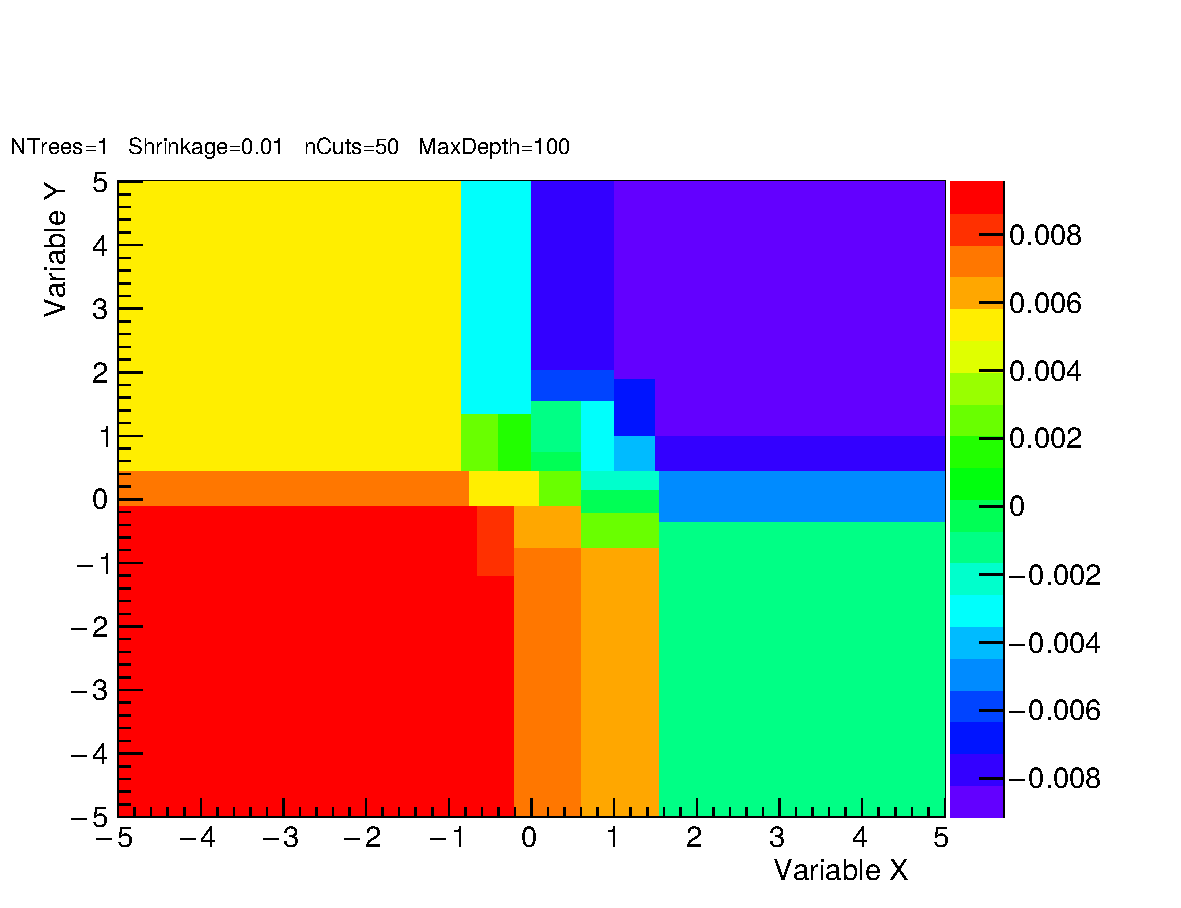
\includegraphics[width=0.85\textwidth]{graphics/tree_depht100.pdf}}
\subfigure[BDT Klassifikation mit 2 Trees]{\label{fig:BDT_nTree2}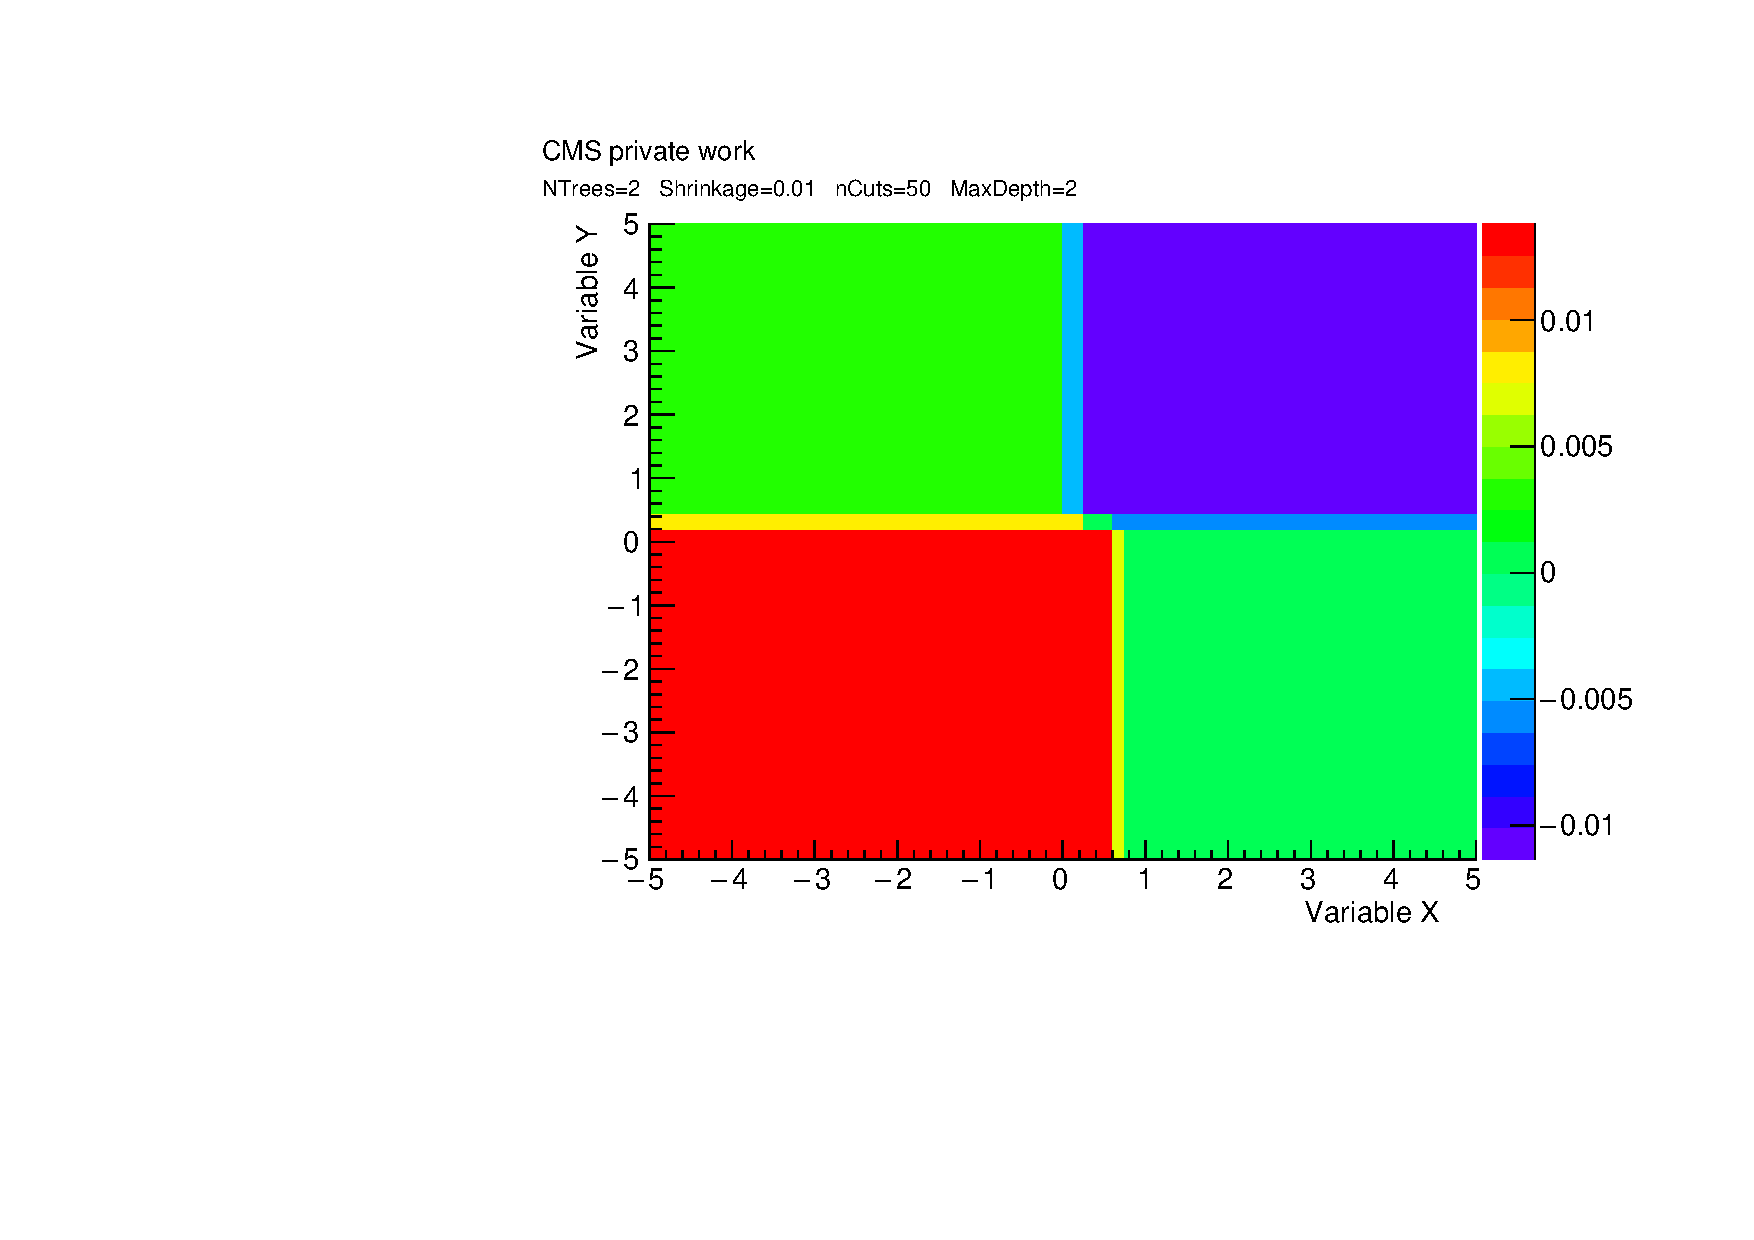
\includegraphics[width=0.85\textwidth]{graphics/tree_depht2_2.pdf}}
\parbox[b]{12cm}{
\caption{Die obere Grafik zeigt die Klassifikation, die mit einem einzelnen Entscheidungsbaum der Tiefe 100 erreicht wird. Signalartige Regionen sind mit positiver Ausgabe in Rott\"onen dargestellt, untergrundartige ergeben eine negative Ausgabe und sind in Blaut\"onen dargestellt. In der unteren Abbildung ist die Klassifikation eines BDT mit zwei B\"aumen der Tiefe zwei zu sehen.}
}
\label{fig:boosting}
\end{figure}

\begin{figure}[tbp]
\centering     %%% not \center
\subfigure[BDT Klassifikation mit 10 Trees]{\label{fig:BDT_nTree10}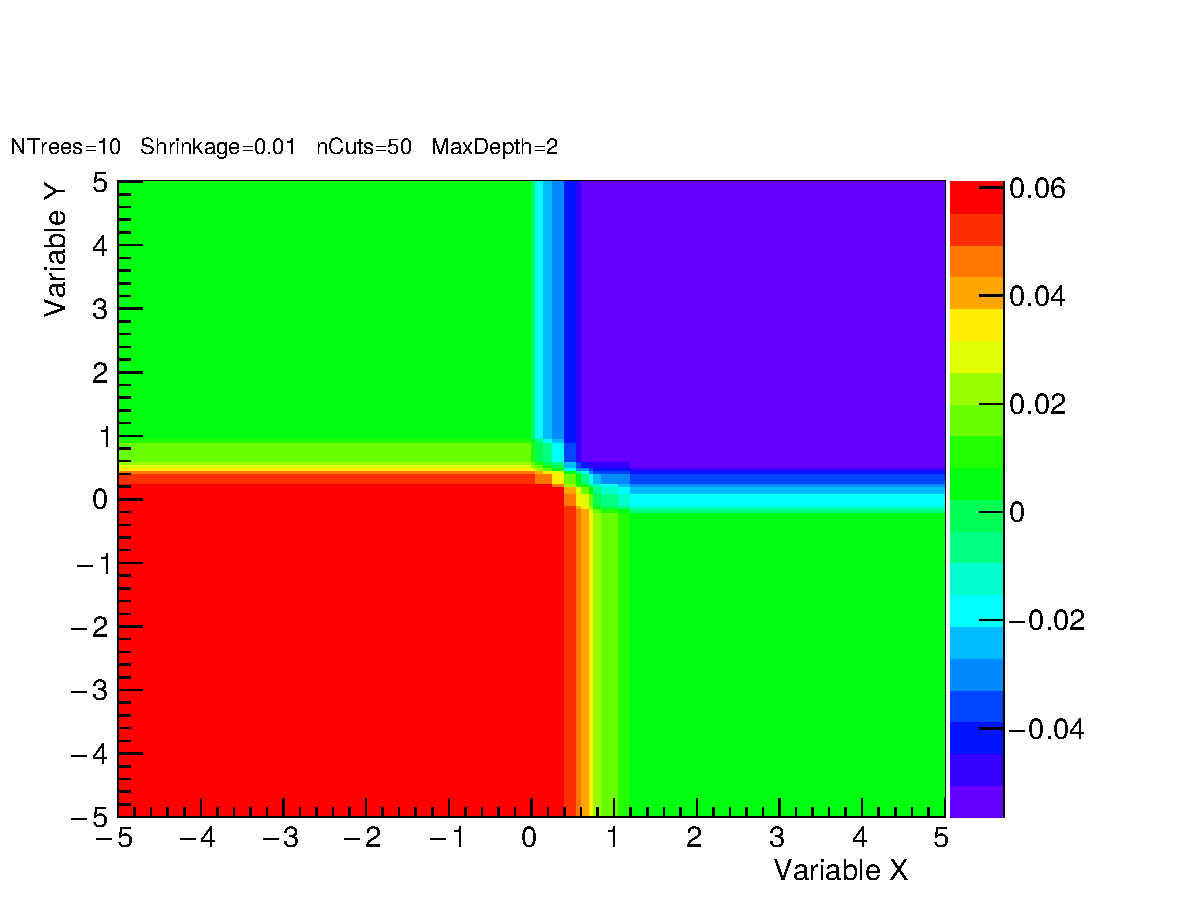
\includegraphics[width=0.85\textwidth]{graphics/tree_depht2_3.pdf}}
\subfigure[BDT Klassifikation mit 100 Trees]{\label{fig:BDT_nTree100}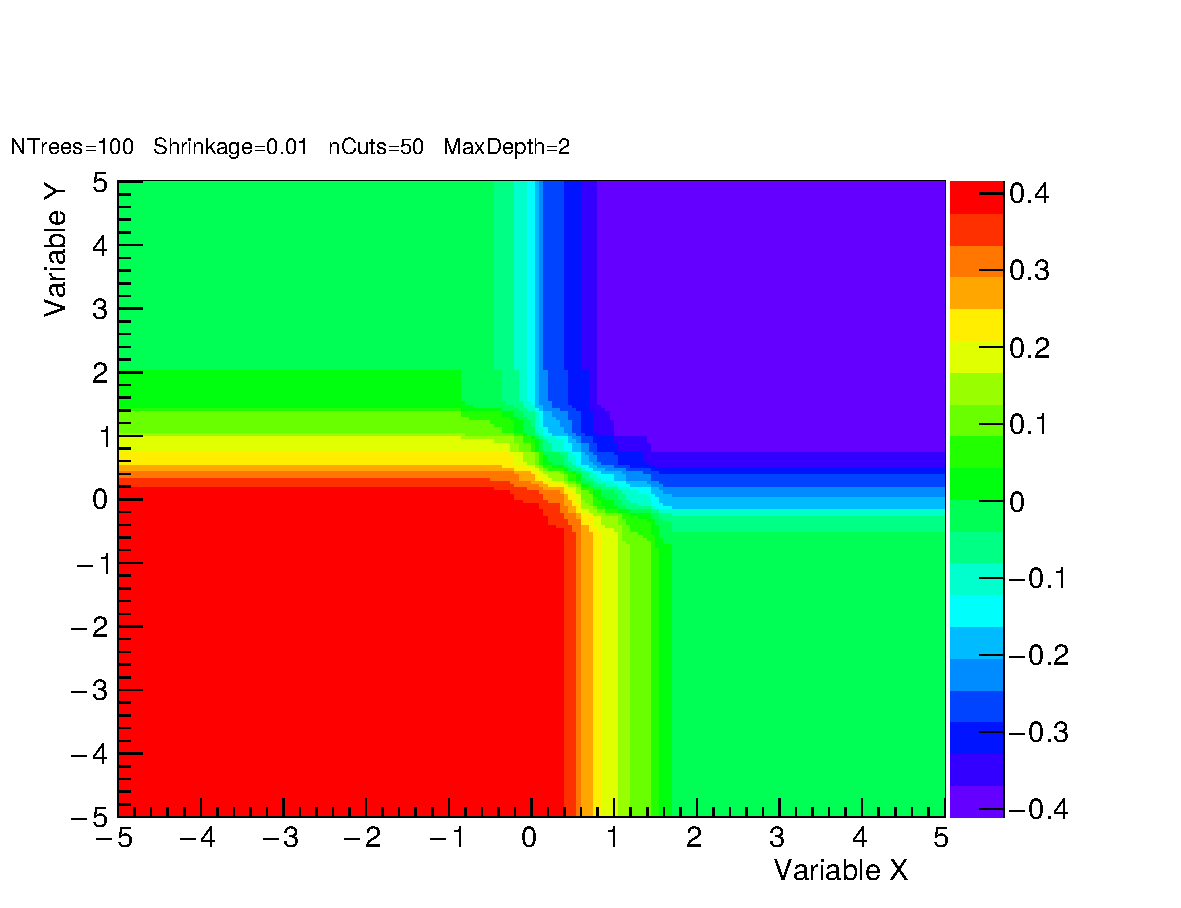
\includegraphics[width=0.85\textwidth]{graphics/tree_depht2_4.pdf}}
\parbox[b]{12cm}{
\caption{Oben ist die Klassifikation eines BDT mit zehn B\"aumen der Tiefe zwei, unten die eines BDT mit 100 B\"aumen der Tiefe zwei abgebildet. Signalartige Regionen sind mit positiver Ausgabe in Rott\"onen dargestellt, untergrundartige ergeben eine negative Ausgabe und sind in Blaut\"onen dargestellt.}
}
\label{fig:boosting}
\end{figure}

%% ===========================
%\subsection{Variieren der Trainingsereignisse (Bagging)}
%\label{ch:Algorithmen:subsec:Bagging}
%% ===========================

%Bagging (aus dem Englischen von bootstrap aggregation abgeleitet) bezeichnet eine Technik die Trainingsereignisse zu variieren. Dabei wird f\"ur jeden trainierten Baum eine zuf\"allige Teilmenge der f\"ur das Training verwendbaren Daten verwendet. Dadurch unterscheiden sich die einzelnen B\"aume voneinander und der Gesamtklassifikator bildet einen Mittelwert der einzelnen schwachen Klassifikatoren. Da Bagging nicht die G\"ute eines Klassifikators verbessern soll, sondern vorallem zum Stabilisieren der Antwort gedacht ist, handelt es sich beim Bagging nicht um einen Boosting-Algorithmus im klassischen Sinn. \cite{Hocker:2007ht}\\
%Der Ansatz des stochastischen Gradient-Boosting vereint Boosting und Bagging.

%% ===========================
\subsection{\"Uberanpassung}
\label{ch:Algorithmen:subsec:overtraining}
%% ===========================

\"Uberanpassung (Overtraining) tritt auf, wenn die MVA-Methode zu wenige Freiheitsgrade zur Verf\"ugung hat, weil zu viele Modellparameter an zu wenige Datenpunkte angepasst werden. So werden statistische Fluktuationen des Trainingsdatensatzes vom Algorithmus gelernt. Dadurch wird zwar die Klassifikation der Trainingsdaten sehr gut, aber die Vorhersage von unbekannten Daten kann deutlich schlechter werden. Diese Verschlechterung bezeichnet man auch als Generalisierungsfehler.

Dies kann beispielsweise auftreten, wenn nur einzelne Ereignisse auf den Knoten eines Entscheidungsbaumes fallen.\\

\begin{figure}[tbp]
\centering     %%% not \center
\subfigure[Streudiagramm von Trainingsdaten]{\label{fig:scat_train_01}\includegraphics[width=0.85\textwidth]{graphics/2d_train_01.pdf}}
\subfigure[Streudiagramm von Testdaten]{\label{fig:scat_test_01}\includegraphics[width=0.85\textwidth]{graphics/2d_test_01.pdf}}
\parbox[b]{12cm}{
\caption{Die vier Streudiagramme zeigen jeweils die Vorhersage auf Trainings- und Testdaten eines Scikit-Learn-BDTs. Richtig klassifizierte Signale sind gelb dargestellt, falsch klassifizierte rot. Richtig identifizierter Untergrund ist t\"urkis gef\"arbt, falsch erkannter lila. In (a) und (b) wurde der BDT mit \num{500} Einzelb\"aumen der Tiefe \num{2} und einer Lernrate von \num{0,05} trainiert, in (c) und (d) mit \num{5000} B\"aumen der Tiefe \num{5} und einer Lernrate von \num{0,5}.}
}
\label{fig:boosting}
\end{figure}

\begin{figure}[tbp]
\centering     %%% not \center
\subfigure[Streudiagramm von Trainingsdaten]{\label{fig:scat_train_02}\includegraphics[width=0.85\textwidth]{graphics/2d_train_02.pdf}}
\subfigure[Streudiagramm von Testdaten]{\label{fig:scat_test_02}\includegraphics[width=0.85\textwidth]{graphics/2d_test_02.pdf}}
\parbox[b]{12cm}{
\caption{Die vier Streudiagramme zeigen jeweils die Vorhersage auf Trainings- und Testdaten eines Scikit-Learn-BDTs. Richtig klassifizierte Signale sind gelb dargestellt, falsch klassifizierte rot. Richtig identifizierter Untergrund ist t\"urkis gef\"arbt, falsch erkannter lila. In (a) und (b) wurde der BDT mit \num{500} Einzelb\"aumen der Tiefe \num{2} und einer Lernrate von \num{0,05} trainiert, in (c) und (d) mit \num{5000} B\"aumen der Tiefe \num{5} und einer Lernrate von \num{0,5}.}
}
\label{fig:boosting}
\end{figure}

In den Abbildungen \ref{fig:scat_train_01} bis \ref{fig:scat_test_02} sind Streudiagramme mit den Klassifikationen von 2 verschiedenen Scikit-Learn-BDT zu sehen. Die Optionen des einen BDTs wurden so gew\"ahlt, dass ein gro\ss er Generalisierungsfehler zu erwarten war (Abbildungen \ref{fig:scat_train_02} und \ref{fig:scat_test_02}). Man erkennt, dass die Vorhersage auf den Trainingsdatensatz besser wurde (Vergleich der Abbildungen \ref{fig:scat_train_01} und \ref{fig:scat_train_02}), die Vorhersage auf den Testdatensatz jedoch deutlich schlechter wurde (Vergleich der Abbildungen \ref{fig:scat_test_01} und \ref{fig:scat_test_02}). Au\ss erdem sind die falsch klassifizierten Ereignisse weit gestreut und nicht mehr in einzelnen Regionen zu finden.
%ist ein Streudiagramm mit der Klassifikation eines stark \"uberangepassten BDTs im Vergleich zu einer Vorhersage ohne Generalisierungsfehler abgebildet. In Abb... und Abb... \todo{BDT output} sind au\ss erdem die BDT-Ausgaben f\"ur unbekannte Testdaten zu sehen.

Es gibt verschiedene Ans\"atze, \"Uberanpassung zu vermeiden. Dazu z\"ahlt das Verwerfen von Entscheidungsbaum\"asten mit zu wenigen Eintr\"agen, gewisserma\ss en das \glqq Abschneiden\grqq~(pruning) des Astes am letzten Knoten mit gen\"ugend Ereignissen. Au\ss erdem ist es \"ublich, den Trainingsdatensatz nochmals in zwei Teile zu spalten. Man spricht dann von Trainings- und Validierungsdatensatz. Mithilfe des Trainingsdatensatzes wird der MVA-Algorithmus trainiert, dann wird die G\"ute des Trainings anhand des Validierungsdatensatzes bestimmt. Sobald man mit der G\"ute der Klassifikation zufrieden ist, kann man den trainierten Algorithmus nutzen, um Vorhersagen f\"ur unbekannte Daten, zum Beispiel die experimentell gemessenen Daten, zu machen.

%% ===========================
\subsection{Variieren der Trainingsereignisse}
\label{ch:Algorithmen:subsec:Bagging}
%% ===========================

Das Variieren der Trainingsereignisse wird als Bagging (aus dem Englischen von bootstrap aggregation abgeleitet) bezeichnet. Dabei wird f\"ur das Training jedes Baumes eine zuf\"allige Teilmenge der f\"ur das Training verwendbaren Daten benutzt. Dadurch unterscheiden sich die einzelnen B\"aume voneinander und der Gesamtklassifikator bildet einen Mittelwert der einzelnen schwachen Klassifikatoren.
%Da Bagging nicht die G\"ute eines Klassifikators verbessern soll, sondern vorallem zum Stabilisieren der Antwort gedacht ist, handelt es sich beim Bagging nicht um einen Boosting-Algorithmus im klassischen Sinn. \cite{Hocker:2007ht}\\
Beim Bagging handelt es sich nicht um einen klassischen Boosting-Algorithmus, da er nicht die Klassifikation verbessern soll, sondern in erster Linie f\"ur eine stabilere Antwort sorgt.\\
Durch Bagging wird der Generalisierungsfehler ebenfalls reduziert.
Der Ansatz des stochastischen Gradient-Boosting vereint Boosting und Bagging \cite{Friedman:2002:SGB:635939.635941}.


%% ===========================
\section{Verwendete Algorithmen zur multivariaten Analyse}
\label{ch:Algorithmen:subsec:Implementationen}
%% ===========================

In diesem Abschnitt werden kurz verschiedene Implementationen von multivariaten Algorithmen vorgestellt, die im weiteren Verlauf der Arbeit miteinander verglichen werden.

%% ===========================
\subsection{Toolkit for Multivariate Analysis in ROOT}
\label{ch:Algorithmen:subsec:TMVA}
%% ===========================

Das Toolkit f\"ur multivariate Datenanalyse in ROOT (TMVA) \cite{Hocker:2007ht} ist ein Softwarepaket, das ins Analyseframework ROOT \cite{ROOT} integriert ist und eine Vielzahl an multivariaten Analysealgorithmen zur Verf\"ugung stellt. Die TMVA-Algorithmen sind speziell f\"ur eine Anwendung in der Teilchenphysik ausgelegt.\\
F\"ur die nachfolgenden Untersuchungen wird der BDT-Algorithmus mit stochastischem Gradient-Boosting der TMVA-Version 4.2.0 in ROOT 6.02/05 verwendet. TMVA BDTs nutzen die binomiale Log-Likelihood-Ausgleichsfunktion
\beq
L(f,y)=\ln{\left(1+\exp{\left(-2f(x)y\right)}\right)}.
\label{eq:tmva_loss}
\eeq


%% ===========================
\subsection{Scikit-Learn -- machine learning in python}
\label{ch:Algorithmen:subsec:sklearn}
%% ===========================

Scikit-Learn ist ein Python-Programm-Paket, das eine Gro\ss zahl von multivariaten Algorithmen zur Verf\"ugung stellt. Im Gegensatz zu TMVA ist das Programmpaket Scikit-Learn nicht speziell f\"ur physikalische Problemstellungen entwickelt, sondern ist auf eine breite Nutzergruppe in allen Bereichen des maschinellen Lernens ausgerichtet \cite{DBLP:journals/corr/abs-1201-0490}.\\
Der in Python 2.7.5 f\"ur die nachfolgenden Untersuchungen verwendete \glqq GradientBoostingClassifier\grqq~der Scikit-Learn-Version 0.18.dev0 nutzt die \glqq Deviance\grqq-Ausgleichsfunktion
\beq
L\left(y,f)\right)=-2\left(y\cdot f-\ln{\left(1+\exp{f}\right)}\right).
\label{eq:deviance}
\eeq

%% ===========================
\subsection{Extreme Gradient Boosting}
\label{ch:Algorithmen:subsec:XGB}
%% ===========================

Extreme Gradient Boosting (XGBoost) \cite{DBLP:journals/corr/ChenG16} ist ein Gradient-Boosting-Algorithmus, der sich stark am theoretischen Modell des Gradient-Boosting von Jerome H. Friedman \cite{Friedman00greedyfunction} orientiert. Er ist f\"ur mehrere Programmierplattformen implementiert, beispielsweise R und Python.\\
Es werden CART-B\"aume verwendet, die in jedem Knoten nicht nur die Trennung der Klassen speichern, sondern jedem Knoten auch einen kontinuierlichen Ausgabewert zuweisen, um die Vorhersage quantitativer zu machen.\\
XGBoost verwendet als Ausgleichsfunktion die mittleren Fehlerquadrate, au\ss erdem ist ein Zusatzterm mit Regularisierungsfunktion implementiert. Insgesamt erh\"alt man f\"ur jeden Boosting-Schritt $t$ eine zu minimierende Zielfunktion mit der Vorhersage $\hat y_i^{t-1}$ des letzten Schrittes und der Summe \"uber alle Trainingsereignisse $i$ von
\beq
F=\sum_{i=1}^n\left[2\left(\hat y_i^{t-1}-y_i\right)f_t+f_t^2\right]+\Omega\left(f_t\right)+Konstante.
\label{eq:xgb_zielfkt}
\eeq
Dabei ist
\beq
\Omega\left(f_t\right)=\gamma T+\frac12\lambda\sum_{j_1}^T w_t^2
\label{eq:complexity}
\eeq
die Komplexit\"at des Baumes mit der Anzahl Endknoten $T$ und den kontinuierlichen Ausgabewerten der B\"aume $w_t$. Die beiden frei w\"ahlbaren Parameter $\lambda$ und $\gamma$ dienen zur Regulierung des Boosting-Algorithmus. Durch Festlegen eines Wertes f\"ur $\gamma$ fordert man eine Mindestreduktion der Ausgleichsfunktion. Wird diese nicht erreicht, wird an diesem Knoten des Baumes keine weitere Unterteilung vorgenommen \cite{xgb_skl_wrapper}. Der Parameter $\lambda$ wird genutzt, um unrentable \"Aste der Entscheidungsb\"aume zu verwerfen. Jedesmal, wenn ein Knoten geteilt werden soll, wird ein Verh\"altnis der Gewichte vor und nach dem Trennen des Knotens berechnet. Ist dieses Verh\"altnis kleiner als $\lambda$, so wird der Ast verworfen \cite{xgb_tree}.\\
Die zu den nachfolgenden Untersuchungen genutzte Version 0.4 von XGBoost wird mit Python 2.7.5 verwendet und wird mithilfe eines Transformationsskriptes f\"ur Scikit-Learn aufgerufen.

%% Theorie.tex
%%
%\usepackage[ngerman]{babel}
%% ==============
\chapter{Vergleich der multivariaten Algorithmen}
\label{ch:vergleich}
%% ==============

%{\bibliographystyle{babalpha-fl}}	% german style
{\bibliographystyle{babunsrt-fl}}

In diesem Kapitel wird zun\"achst erl\"autert, anhand welcher Kriterien die verwendeten Algorithmen miteinander verglichen werden k\"onnen. Anschlie\ss end werden die Algorithmen auf zwei verschiedene S\"atze von CMS-Simulationsdaten angewandt und die Ergebnisse verglichen.

%% ===========================
\section{Vergleichbarkeit der Algorithmen}
\label{ch:Vergleich:sec:Vergleichbarkeit}
%% ===========================

Bevor die verschiedenen Implementationen der Algorithmen verglichen werden k\"onnen, m\"ussen zun\"achst einige Vergleichskriterien festgelegt werden. Au\ss erdem muss \"uberpr\"uft werden, inwieweit sich die Parameter der Algorithmen unterscheiden.\\
In Tabelle \ref{tab:parameter} sind die Einstellungsm\"oglichkeiten der drei Algorithmen dargestellt.

\begin{table}[tbp]\parbox{12cm}{
  \caption[Algorithmenparameter]{Tabelle mit einstellbaren Parametern der verschiedenen Algorithmen}% {\rm \cite{Agashe:2014kda}}
  }\label{tab:parameter}
  \begin{center}
  \begin{tabular}{p{3.75cm}p{2.75cm}p{2.25cm}p{4.5cm}}
  \hline
  {\bf TMVA} & {\bf scikit-learn} & {\bf XGBoost} & {\bf Funktion} \\
  \hline \hline
     NTrees	& n\_estimators & n\_estimators & Anzahl der Entscheidungsb\"aume \\
     Shrinkage	& learning\_rate & learning\_rate & Lernrate des Gradient Boosting \\
     MaxDepth & max\_depth & max\_depth & Tiefe der Entscheidungsb\"aume\\
     nCuts & -- & -- & Anzahl an getesteten Schnitten\\ 
  	 MinNodeSize & min\_samples\_leaf & reg\_lambda & Minimalanzahl Ereignisse pro Knoten\\ 
  	 BaggedSampleFraction & subsample & subsample & Gr\"o\ss e der Teilmengen des Trainingsdatensatzes f\"ur Bagging\\                     
  \hline
  \end{tabular}
  \end{center}
\end{table}

Die Lernrate, die Anzahl an Entscheidungsb\"aumen sowie die Tiefe der B\"aume haben bei allen drei Algorithmen die gleiche Funktion. Die Anzahl der zu testenden Schnitte ist nur in TMVA regelbar. Dies k\"onnte daran liegen, dass in TMVA viele Berechnungen mithilfe von der ROOT implementierten Histogramme durchgef\"uhrt werden, w\"ahrend Scikit-Learn Arrays verwendet, die keine Schnitte ben\"otigen sondern eine kontinuierliche \"Uberpr\"ufung der Ausgabe erm\"oglichen. 

Die minimale Anzahl an Ereignissen pro Knoten legt fest, ab wann ein Entscheidungsbaum beschnitten werden soll. In TMVA wird dies \"uber einen Prozentsatz des Trainingsdatensatzes festgelegt, w\"ahrend in Scikit-Learn ein Absolutwert genutzt wird. In XGBoost wird dies durch einen Vergleich der Ereignisgewichte erreicht.

Um nur die Gr\"o\ss e der zuf\"alligen Teilmenge einzustellen, die jeder Entscheidungsbaum durch Bagging zum Training nutzt, dient die \glqq BaggedSampleFraction\grqq~in TMVA sowie das \glqq subsample\grqq in Scikit-Learn und XGBoost. Beide sind Parameter im Bereich zwischen 0 und 1 und werden mit der Gesamtanzahl der Trainingsereignisse multipliziert, um die Anzahl der Ereignisse pro Baum zu erhalten.

Au\ss erdem m\"ussen zun\"achst Kriterien gefunden werden, anhand derer die BDT-Ausgaben miteinander verglichen werden k\"onnen. In dieser Arbeit werden ROC-Kurve (Abschnitt~\ref{ch:Vergleich:subsec:ROC}) sowie das Integral der ROC-Kurven zum Vergleich der Klassifikationsqualit\"at und der Kolmogorov-Smirnov-Test (Abschnitt \ref{ch:Vergleich:subsec:KSTest}) zur Untersuchung, ob ein Generalisierungsfehler vorliegt, verwendet.

%% ===========================
\subsection{ROC-Kurve}
\label{ch:Vergleich:subsec:ROC}
%% ===========================

Receiver-Operating-Characteristic-Kurven (ROC-Kurven) sind Kennlinien, die sich als n\"utzliche Technik zur Visualisierung der G\"ute eines Klassifikators herausgestellt haben.

In einem ROC-Graphen wird die Sensitivit\"at (Richtig-Positiv-Rate) \"uber der Spezifit\"at (1 - Falsch-Positiv-Rate) aufgetragen. Dabei ist die Sensitivit\"at definiert als
\beq
tpr = \frac{\text{korrekt~klassifizierte~Signalereignisse}}{\text{Gesamtanzahl~Signalereignisse}}
\label{eq:TPR}
\eeq
und die Spezifit\"at als
\beq
1-fpr = 1-\frac{\text{falsch~klassifizierte~Untergrundereignisse}}{\text{Gesamtanzahl~Untergrundereignisse}}.
\label{eq:1-FPR}
\eeq
%
Manchmal wird auch die Richtig-Positiv-Rate \"uber der Falsch-Positiv-Rate aufgetragen. Dadurch erh\"alt man eine ansteigende ROC-Kurve. An den Eigenschaften der ROC-Kurve \"andert das allerdings nichts.

F\"ur jede diskrete Unterscheidung wird ein Punkt der ROC-Kurve erzeugt. Dieser Punkt besteht aus einem Wertepaar der Form $((1-fpr),tpr)$. F\"ur einen Entscheidungsbaum der Tiefe zwei erh\"alt man also drei Punkte. Au\ss erdem enth\"alt jede ROC-Kurve die Punkte $(0,1)$, was bedeutet, dass kein Ereignis als Signal eingestuft wird und $(1,0)$, an dem alle Ereignisse als Signal eingestuft werden. Diese Punkte werden durch Geraden verbunden, um eine gemittelte Kurve zu erhalten.\\
Die schlechtest m\"ogliche Klassifikation w\"urde eine Gerade zwischen diesen beiden Punkten ergeben und entspricht einer zuf\"alligen Einteilung in Signal und Untergrund. Eine perfekte Klassifikation w\"urde den Punkt $(1,1)$ ergeben. Somit w\"urde man eine Fl\"ache unter der ROC-Kurve von eins erhalten. Diese Fl\"ache wird ebenfalls als Vergleichskriterium f\"ur Klassifikatoren benutzt. Man nennt sie auch ROC-Integral oder ROC-AUC (f\"ur area under curve) \cite{ROC_Graphs}.

\begin{figure}[tbp]
\centering     %%% not \center
\subfigure[ROC-Kurve eines Baumes der Tiefe zwei]{\label{fig:ROC_1}\includegraphics[width=0.85\textwidth]{graphics/ROC_1.pdf}}
\subfigure[ROC-Kurve eines BDT mit 1000 B\"aumen der Tiefe zwei]{\label{fig:ROC_1000}\includegraphics[width=0.85\textwidth]{graphics/ROC_1000.pdf}}
\parbox[b]{12cm}{
\caption{Oben sieht man die ROC-Kurve einer Klassifikation mit einem einzelnen Baum der Tiefe zwei. Darunter ist eine ROC-Kurve eines BDTs mit 1000 B\"aumen der Tiefe zwei abgebildet.}}
\end{figure}

In Abbildung \ref{fig:ROC_1} ist eine ROC-Kurve der Klassifikation eines einzelnen Entscheidungsbaumes zu sehen, man erkennt die drei Punkte der ROC-Kurve. In Abbildung \ref{fig:ROC_1000} ist eine ROC-Kurve der Klassifikation eines BDTs mit 1000 B\"aumen der Tiefe zwei zu sehen. Die Kurve wird deutlich runder, da mehr Unterscheidungen getroffen werden k\"onnen und somit mehr Wertepaare f\"ur die ROC-Kurve erzeugt werden. Au\ss erdem wird die Fl\"ache unter der Kurve gr\"o\ss er, was auf die bessere Klassifikation hinweist.
Erzeugt wurden beide ROC-Kurven mit einer Pythonfunktion anhand einer Klassifikation des Beispiels aus Abschnitt \ref{ch:Algorithmen:sec:BDT} mit Scikit-Learn.

%% ===========================
\subsection{Kolmogorov-Smirnov-Test}
\label{ch:Vergleich:subsec:KSTest}
%% ===========================

Der Kolmogorov-Smirnov-Test ist ein statistischer Test, mit dem gepr\"uft wird, wie gut zwei verschiedene Verteilungsfunktionen \"ubereinstimmen.\\
Um eine Klassifikation eines BDTs auf \"Uberanpassung zu testen wird jeweils eine Verteilungsfunktion der BDT-Ausgabe auf den Trainingsdatensatz und auf einen unabh\"angigen Testdatensatz erstellt. Dies geschieht indem man die BDT-Ausgaben $x_i$ der Ereignisse $i$ der Gr\"o\ss e nach sortiert. Die Verteilungsfunktionen sind dann
\beq
F_{\mathrm{train}}(x) = \frac{\text{Anzahl~der~x$_i$-Werte} \leq x}{n}
\label{eq:CDF_train}
\eeq
und f\"ur den Testdatensatz entsprechend.\\
Gesucht wird die gr\"o\ss te Differenz zwischen diesen beiden Verteilungen
\beq
t = \sqrt{n}\cdot\max\left|F_{\mathrm{train}}(x)-F_{\mathrm{test}}(x)\right|.
\label{eq:KSTest}
\eeq
Je kleiner dieser Wert ist, desto besser stimmen die Verteilungsfunktionen \"uberein \cite{Blobel}. Wenn dieser Wert f\"ur Test- und Trainingsdaten gro\ss~wird, so ist dies ein Hinweis darauf, dass ein Generalisierungsfehler vorliegt.

Oft wird auch die Wahrscheinlichkeit berechnet, einen Wert $\leq t_0$ f\"ur die Testgr\"o\ss e $t$ zu erhalten. In diesem Fall sind die Verteilungen bei kleinen Wahrscheinlichkeiten nicht kompatibel. Diese Wahrscheinlichkeit wird zum Beispiel von der in ROOT implementierten Funktion des KS-Tests als R\"uckgabewert genutzt \cite{ROOT:TH1F}.

%% ===========================
\section{Verwendete Datens\"atze}
\label{ch:Vergleich:sec:Daten}
%% ===========================

Um die multivariaten Algorithmen zu vergleichen werden diese auf CMS-Simulationsdaten angewendet. Als Untergrunddatensatz wird ein Datensatz mit simulierten \ttb-Ereignissen, mit in Powheg \cite{Frixione:2007vw} simuliertem Matrixelement und mit Pythia \cite{Sjostrand2015159} simuliertem Partonschauer, verwendet. Die offizielle Bezeichnung des Simulationsdatensatzes lautet {\it/TT TuneCUETP8M1 13TeV-powheg-pythia8/RunIIFall15MiniAODv2-PU25nsData2015v1-76X mcRun2 asymptotic RunIIFall15DR76 v0 ext3-v1/MINIAODSIM }.\\
Als Signaldatensatz wird ein simulierter \ttH-Datensatz verwendet, bei dem das Matrixelement ebenfalls mit Powheg und der Partonschauer mit Pythia simuliert wurde. Die offizielle Bezeichnung lautet \begin{it}/ttHTobb M125 13TeV powheg pythia8/RunIIFall15MiniAODv1-PU25nsData2015v1 76X mcRun2 asymptotic v12v1/MINIAODSIM\end{it}.\\
Beide Datens\"atze wurden f\"ur eine Schwerpunktsenergie von \num{13} \si{\tera\electronvolt} simuliert. Danach wurden die Prozesse auf ihre Standardmodell-Wirkungsquerschnitte umgewichtet.

Wie in Abschnitt \ref{ch:Experiment:sec:ttH} beschrieben, unterteilt man die \ttH-Analyse in verschiedene Kategorien. Der Vergleich der multivariaten Algorithmen wird f\"ur zwei dieser Kategorien durchgef\"uhrt. F\"ur die erste Auswahl wird genau ein Lepton mit einem Transversalimpuls von $p_T\geq \num{30}~\si{\giga\electronvolt}$ und mindestens sechs Jets mit $p_T\geq \num{30}~\si{\giga\electronvolt}$, von denen vier oder mehr als b-Quark identifiziert wurden, gefordert (6-Jet-4-B-Tag). Alle Ereignisse mit gerader Ereignisidentifikationsnummer werden zum Trainieren der BDTs verwendet, die mit ungerader zum Testen der Klassifikation. Dadurch erh\"alt man einen \ttH-Trainingsdatensatz mit 17026 Ereignissen und einen \ttb-Trainingsdatensatz mit 42378 Ereignissen.

F\"ur die zweite Auswahl wird ebenfalls genau ein Lepton mit $p_T\geq \num{30} \si{\giga\electronvolt}$ und mindestens sechs Jets mit $p_T\geq \num{30}~\si{\giga\electronvolt}$ gefordert, allerdings sollen nur zwei der Jets zu b-Quarks geh\"oren (6 Jets und 2 B-Tags). Trainings- und Testdatens\"atze werden wieder anhand gerader und ungerader Ereignisse unterschieden. Dadurch erh\"alt man insgesamt 1901054 Untergrundereignisse und 38074 Signalereignisse als Trainingsdaten, damit ist das Signal zu Untergrundverh\"altnis viel kleiner als in der Kategorie mit sechs Jets und mindestens vier B-Tags. Allerdings wurden nur 2364 Signalereignisse und 119823 Untergrundereignisse verwendet, um das Verhalten der Algorithmen bei geringer Statistik zu untersuchen. 

Als trennende Variablen werden in der Kategorie mit sechs Jets und mindestens vier B-Tags\\
{\it Evt\_Deta\_JetsAverage, avg\_btag\_disc\_btags, avg\_dr\_tagged\_jets, dEta\_fn, h3, maxeta\_jet\_tag, pt\_all\_jets\_over\_E\_all\_jets, sphericity, BDT\_common5\_output, Evt\_CSV\_Average\_Tagged} und {\it Evt\_Deta\_TaggedJetsAverage}\\verwendet.

In der Kategorie mit sechs Jets und zwei B-Tags werden \\ {\it h1, avg\_dr\_tagged\_jets, sphericity, third\_highest\_btag, h3, HT, Mlb, fifth\_highest\_CSV} und {\it fourth\_highest\_btag} als trennende Variablen verwendet.\\
%{\it Evt\_Deta\_JetsAverage,avg\_btag\_disc\_btags,avg\_dr\_tagged\_jets, dEta\_fn, h3, maxeta\_jet\_tag, pt\_all\_jets\_over\_E\_all\_jets, \\sphericity, \\BDT\_common5\_output, Evt\_CSV\_Average\_Tagged und Evt\_Deta\_TaggedJetsAverage}\\verwendet.st\_btag}\\als trennende Variablen verwendet.
Alle diese Variablen haben eine physikalische Bedeutung, auf diese wird hier allerdings nicht n\"aher eingegangen, da sie f\"ur den Vergleich der multivariaten Algorithmen nicht relevant sind. Details k\"onnen in \cite{CMS-PAS-HIG-16-004} nachgeschlagen werden.

%% ===========================
\section{Vorgehensweise w\"ahrend der Untersuchung}
\label{ch:Vergleich:sec:Vorgehensweise}
%% ===========================

Wie in Tabelle \ref{tab:parameter} gezeigt, gibt es f\"ur den TMVA-Parameter nCuts keine Entsprechung in Scikit-Learn und XGBoost. Daher soll zun\"achst untersucht werden welchen Einfluss dieser Parameter hat. Dazu wird der TMVA-Algorithmus mehrfach auf den Simulationsdatensatz der 6-Jet-4-B-Tag-Kategorie angewendet und nur der Parameter nCuts variiert. Die \"ubrigen Parameter sind jeweils NTrees=1000, MinNodeSize=2.5\%, Shrinkage=0.01, BaggedSampleFraction=0.6 und MaxDepth=2.
In Tabelle \ref{tab:nCuts} sind die Ergebnisse dieser Trainings dargestellt.

\begin{table}[tbp]\parbox{12cm}{
  \caption[Variation des TMVA-nCuts-Parameters]{Tabelle mit ROC-Integral und Wahrscheinlichkeit des Kolmogorov-Smirnov-Test f\"ur Signal- und Untergrundverteilung von TMVA-Trainings mit den festen Einstellungen NTrees=1000, MinNodeSize=2.5\%, Shrinkage=0.01, BaggedSampleFraction=0.6, MaxDepth=2 und in Abh\"angigkeit des Parameters nCuts}% {\rm \cite{Agashe:2014kda}}
  }\label{tab:nCuts}
  \begin{center}
  \begin{tabular}{llll}
  \hline
  nCuts & ROC-Integral & P(KS) Signal & P(KS) Untergrund\\
  \hline
  \num{2} & \num{0,730} & \num{0,34} & \num{0,99}\\
 \num{20} & \num{0,734} & \num{0,19} & \num{1}\\
 \num{50} & \num{0,734} & \num{0,14} & \num{1}\\
\num{500} & \num{0,734} & \num{0,27} & \num{1}\\
  \hline
  \end{tabular}
  \end{center}
\end{table}

Solange nCuts ausreichend gro\ss~gew\"ahlt wird, hat dieser Parameter bei diesem Datensatz also nur einen geringen Einfluss auf die Klassifikation. Im Folgenden wird daher immer nCuts=\num{50} verwendet.

Als n\"achstes wird versucht die anderen Parameter sinnvoll einzugrenzen. Da die BaggedSampleFraction beziehungsweise das subsample nur zur Stabilisierung des Klassifikators gedacht ist, wird diese auf den Standardwert aus TMVA, BaggedSampleFraction=\num{0,6}, gesetzt.\\
Wie in \cite{SWB-307748006} beschrieben, haben bisherige Erfahrungen gezeigt, dass BDTs die besten Resultate liefern, wenn die Anzahl an Knoten der einzelnen B\"aume zwischen vier und acht liegt, eine Lernrate unter \num{0,1} verwendet wird und die Anzahl der Entscheidungsb\"aume so gro\ss~wie m\"oglich gew\"ahlt wird, ohne in einen Bereich der \"Uberanpassung zu gelangen.\\
Der vorgeschlagenenen Anzahl an Knoten pro Baum entspricht eine Tiefe von zwei, daher wird die Tiefe ebenfalls auf zwei festgesetzt.

Die Lernrate und die Anzahl von Entscheidungsb\"aumen beeinflussen sich gegenseitig. So kann man beispielsweise nicht beiden Parametern einen hohen Wert zuweisen, ohne einen hohen Generalisierungsfehler in Kauf zu nehmen. W\"ahlt man jedoch eine kleine Lernrate, so kann man die Anzahl an Entscheidungsb\"aumen h\"oher w\"ahlen und den Generalisierungsfehler trotzdem gering halten. W\"ahrend einiger Tests stellte sich heraus, dass die besten Ergebnisse mit einer Lernrate unter \num{0,01} zustande kommen.

Obwohl diese beiden Parameter in den drei Implementierungen der Algorithmen gleich definiert sind, kann es durch die Unterschiede der Algorithmen auch unterschiedliche Ergebnisse bei gleicher Parameterwahl geben. Aus diesen Gr\"unden werden die Algorithmen nicht anhand eines einzelnen Trainings mit gleichen Parametern verglichen, sondern die Lernrate und die Anzahl B\"aume wird in einem sinnvollen Bereich variiert. Anschlie\ss end werden die besten Ergebnisse der drei Klassifikatoren miteinander verglichen.

\begin{table}[tbp]\parbox{12cm}{
  \caption[TMVA 6j4t Ergebnisse]{Tabelle mit Ergebnissen des TMVA-Algorithmus f\"ur verschiedene Parametereinstellungen in der 6 Jets 4 B-Tags Kategorie.\\In den ersten beiden Spalten sind die verwendete Anzahl der B\"aume und die verwendete Lernrate, in den weiteren Spalten ROC-Integral und die Wahrscheinlichkeiten des Kolmogorov-Smirnov-Tests f\"ur Signal- und Untergrundverteilung eingetragen.}% {\rm \cite{Agashe:2014kda}}
  }\label{tab:tmva_6j4t}
  \begin{center}
  \begin{tabular}{lllll}
  \hline
  NTrees & Shrinkage & ROC-Integral & P(KS) Signal & P(KS) Untergrund\\
  \hline
 \num{1500}  & \num{0,001}   & \num{0,729} & \num{0,2}  & \num{0,34}\\
 \num{1500}  & \num{0,0028}  & \num{0,732} & \num{0,28} & \num{0,97}\\
 \num{1500}  & \num{0,0046}  & \num{0,733} & \num{0,21} & \num{0,99}\\
 \num{1500}  & \num{0,0064}  & \num{0,734} & \num{0,22} & \num{0,99}\\
 \num{1500}  & \num{0,0082}  & \num{0,734} & \num{0,11} & \num{1}\\
 \num{1700}  & \num{0,001}   & \num{0,729} & \num{0,22} & \num{0,86}\\
 \num{1700}  & \num{0,0028}  & \num{0,732} & \num{0,23} & \num{0,99}\\
 \num{1700}  & \num{0,0046}  & \num{0,733} & \num{0,19} & \num{0,99}\\
 \num{1700}  & \num{0,0064}  & \num{0,734} & \num{0,17} & \num{0,99}\\
 \num{1700}  & \num{0,0082}  & \num{0,734} & \num{0,17} & \num{0,98}\\
 \num{1900}  & \num{0,001}   & \num{0,73}  & \num{0,26} & \num{0,78}\\
 \num{1900}  & \num{0,0028}  & \num{0,732} & \num{0,26} & \num{0,99}\\
 \num{1900}  & \num{0,0046}  & \num{0,733} & \num{0,2}  & \num{0,98}\\
 \num{1900}  & \num{0,0064}  & \num{0,734} & \num{0,16} & \num{1}\\
 \num{1900}  & \num{0,0082}  & \num{0,734} & \num{0,23} & \num{0,98}\\
 \num{2100}  & \num{0,001}   & \num{0,73}  & \num{0,23} & \num{0,72}\\
 \num{2100}  & \num{0,0028}  & \num{0,732} & \num{0,23} & \num{0,99}\\
 \num{2100}  & \num{0,0046}  & \num{0,734} & \num{0,17} & \num{0,98}\\
 \num{2100}  & \num{0,0064}  & \num{0,734} & \num{0,18} & \num{0,99}\\
 \num{2100}  & \num{0,0082}  & \num{0,735} & \num{0,29} & \num{0,94}\\
 \num{2300}  & \num{0,001}   & \num{0,730} & \num{0,26} & \num{0,9}\\
 \num{2300}  & \num{0,0028}  & \num{0,733} & \num{0,21} & \num{0,98}\\
 \num{2300}  & \num{0,0046}  & \num{0,734} & \num{0,15} & \num{1}\\
 \num{2300}  & \num{0,0064}  & \num{0,734} & \num{0,2}  & \num{1}\\
 \num{2300}  & \num{0,0082}  & \num{0,735} & \num{0,20} & \num{0,97}\\
  \hline
  \end{tabular}
  \end{center}
\end{table}

In Tabelle \ref{tab:tmva_6j4t} sind die Resultate der mit TMVA in der Kategorie mit 6 Jets und 4 B-Tags durchgef\"uhrten Trainings dargestellt. Die Tabellen mit den Resultaten der anderen Algorithmen und denjenigen mit den Untersuchungen in der Kategorie mit 6 Jets und 2 B-Tags finden sich im Anhang.

Man erkennt, dass das ROC-Integral f\"ur gro\ss e Lernraten und eine hohe Anzahl von Entscheidungsb\"aumen zunimmt, allerdings nur geringf\"ugig. Die besten Ergebnisse liefern die BDTs mit einer Lernrate von \num{0,0082} und 2100 beziehungsweise 2300 B\"aumen. Die Wahrscheinlichkeiten der Kolmogorov-Smirnov-Tests befinden sich f\"ur die Signalverteilungen im Bereich von \num{0,11} bis \num{0,29}. Aus Erfahrungen hat sich gezeigt, dass diese Werte nicht auf einen gravierenden Generalisierungsfehler hindeuten. Dies w\"are der Fall wenn die Wahrscheinlichkeit gegen Null geht. Daher wird jeweils ein Wert gr\"o\ss er \num{0,1} gefordert.

Wie bei den Trainings mit TMVA wird die Fl\"ache unter der ROC-Kurve gr\"o\ss er, je h\"oher die Lernrate und die Anzahl der Entscheidungsb\"aume sind. Allerdings werden die Wahrscheinlichkeiten des Kolmogorov-Smirnov-Tests deutlich kleiner als bei den TMVA-Trainings. So fallen relativ viele unterhalb der bei \num{0,1} gesetzten Marke und werden nicht ber\"ucksichtigt. Aufgrund dessen ist die beste Einstellung, die f\"ur Scikit-Learn gefunden wurde, eine Lernrate von \num{0,0046} und \num{2300} Entscheidungsb\"aumen.

Auch XGBoost erreicht die besten Ergebnisse mit gr\"o\ss eren Lernraten und vielen Entscheidungsb\"aumen. Hier liegen die Wahrscheinlichkeiten aus dem Kolmogorov-Smirnov-Tests weiter auseinander als bei den anderen beiden Algorithmen. Es gibt auch Trainings, die aufgrund des schlechten Ergebnisses beim Kolmogorov-Smirnov-Test nicht ber\"ucksichtigt werden, mit drei sind dies aber deutlich weniger als bei Scikit-Learn. Das beste Ergebnis wird mit einer Lernrate von \num{0,0064} und \num{2300} Entscheidungsb\"aumen erreicht.

\begin{figure}[tbp]
\centering     %%% not \center
\subfigure[ROC-Kurven der jeweils besten Trainings]{\label{fig:ROC_6j4t}\includegraphics[width=0.85\textwidth]{graphics/ROC_6j4t.pdf}}
\subfigure[BDT-Ausgabe der jeweils besten Trainings]{\label{fig:BDTout_6j4t}\includegraphics[width=0.85\textwidth]{graphics/BDToutput_6j4t.pdf}}
\parbox[b]{12cm}{
\caption{Oben sind die ROC-Kurven der jeweils besten Trainings in der Kategorie mit mindestens sechs Jets und mindestens vier B-Tags abgebildet, darunter jeweils die BDT-Ausgaben.}}
\end{figure}

In Abbildung \ref{fig:ROC_6j4t} sind die ROC-Kurven der jeweils besten Trainings abgebildet. Sie sind nahezu identisch. In Abbildung \ref{fig:BDTout_6j4t} sind die BDT-Ausgaben der besten Training zu sehen. Man sieht, dass f\"ur jeden Klassifikator die BDT-Ausgabe etwas anders definiert ist. XGBoost gibt beispielsweise die Signalwahrscheinlichkeit f\"ur ein Ereignis zur\"uck, w\"ahrend TMVA einen Wert zwischen $\pm1$ zur\"uckgibt.

Generell sind die ROC-Integrale in der Kategorie mit sechs Jets und zwei B-Tags kleiner als in der Kategorie mit sechs Jets und vier B-Tags. Dies liegt vor allem daran, dass die Kategorie stark untergrunddominiert ist, also nur wenige Signalereignisse auf viele Untergrundereignisse fallen.

Die Fl\"ache unter der ROC-Kurve ist in dieser Kategorie mit Scikit-Learn immer etwa \num{0,01} gr\"o\ss er als bei TMVA. Allerdings f\"allt der Kolmogorov-Smirnov-Test sehr schlecht aus, allerdings kann dies \"uber andere Einstellungen, beispielsweise bei min\_samples\_leaf, noch verbessert werden.

XGBoost schneidet in dieser Kategorie ebenfalls besser ab als TMVA und der Kolmogorov-Smirnov-Test f\"allt etwas besser aus als bei Scikit-Learn.

\begin{figure}[tbp]
\centering     %%% not \center
\subfigure[ROC-Kurven der jeweils besten Trainings]{\label{fig:ROC_6j4t}\includegraphics[width=0.85\textwidth]{graphics/ROC_6j2t.pdf}}
\subfigure[BDT-Ausgabe der jeweils besten Trainings]{\label{fig:BDTout_6j4t}\includegraphics[width=0.85\textwidth]{graphics/BDToutput_6j2t.pdf}}
\parbox[b]{12cm}{
\caption{In der oberen Grafik sind die ROC-Kurven der jeweils besten Trainings in der Kategorie mit mindestens sechs Jets und zwei B-Tags abgebildet, in der unteren jeweils die normierten BDT-Ausgaben.}}
\end{figure}

In Abbildung \ref{fig:ROC_6j4t} sind die ROC-Kurven der jeweils besten Trainings gezeigt. In der Kategorie mit mindestens sechs Jets und zwei B-Tags ist ein Unterschied zwischen den ROC-Kurven zu erkennen. In Abbildung \ref{fig:BDTout_6j4t} sind die BDT-Ausgaben abgebildet. Aufgrund des geringen Signal-zu-Untergrund-Verh\"altnisses wurden die Verteilungen normiert.

Urspr\"unglich sollte auch die zum Trainieren der BDTs ben\"otigte Zeit verglichen werden. Allerdings wurden alle Trainings auf einem Rechencluster durchgef\"uhrt. Je nach Auslastung des Clusters varierten die Trainingszeiten, daher ist kein objektiver Vergleich m\"oglich. Generell nimmt die Zeit, die man f\"ur ein Training ben\"otigt, mit der Zahl der Entscheidungsb\"aume zu, weswegen eine Abw\"agung von Klassifikationseffizienz zur Trainingsdauer n\"otig ist.

%% ===========================
\section{Nutzbarkeit der Algorithmen in der \ttH-Analyse}
\label{ch:Vergleich:sec:ttH}
%% ===========================

In diesem Abschnitt soll gekl\"art werden, inwieweit sich die getesteten Algorithmen in der \ttH-Analyse einsetzen lassen.

Eine der wichtigsten Anforderungen an die multivariaten Algorithmen in der \ttH-Analyse ist die M\"oglichkeit den Klassifikator zu speichern, sodass die im Detektor gemessenen Daten mit einem zuvor auf Simulationsdaten trainierten Klassifikator analysiert werden k\"onnen.

Bei dem zur Zeit verwendeten TMVA BDT werden die Schnitte und Gewichte des Trainings in eine Textdatei (.xml-Format) gespeichert. Diese kann mithilfe einer eigenen Klasse, dem TMVA-Reader geladen werden. Durch die geladenen BDT-Gewichte, kann der TMVA-Reader dann eine Vorhersage f\"ur unbekannte Daten \"ubernehmen.

In Scikit-Learn besteht die M\"oglichkeit den Klassifikator direkt mit dem Python-Paket \glqq pickle\grqq~ als Packing-List-File (.pkl-Datei) zu Speichern und wieder zu laden. Der Klassifikator stellt hier selbst Funktionen bereit, mit denen Vorhersagen auf unbekannte Daten erstellt werden k\"onnen, ohne dass eine separates Objekt erstellt werden muss.

Bei der mit dem Transformationsskript aufgerufenen Implementation von XGBoost besteht die gleiche M\"oglichkeit, den Klassifikator zu speichern. Allerdings war dies w\"ahrend der Tests aufgrund von Kompatibilit\"atsproblemen nicht m\"oglich.

Dies f\"uhrt zu einem weiteren wichtigen Punkt, der beachtet werden muss. In der CMS-Kollaboration wird das CMSSW Application Framework \cite{CMSSW} genutzt. Dies kann man sich als eine Art virtuelles System vorstellen, auf dem in einem modularen Aufbau Software bereitgestellt wird. W\"ahrend ROOT inklusive TMVA in CMSSW integriert sind, wird zur Zeit weder Scikit-Learn noch XGBoost bereitgestellt. F\"ur die Untersuchungen im Rahmen dieser Arbeit wurde teils auf Softwaremodule des CMSSW-Framework zur\"uckgegriffen, die mit lokalen Installationen von Scikit-Learn und XGBoost erg\"anzt wurden. Allerdings war die Installation und Konfiguration kompliziert.

Dies stellt derzeit einen klaren Nachteil f\"ur Scikit-Learn und XGBoost dar. Solange diese Pakete nicht ins CMSSW-Framework integriert werden, ist eine Nutzung in der \ttH-Analyse nicht sinnvoll.
%% zusammenfassung.tex
%%

%% ==================
\chapter{Fazit und Ausblick}
\label{ch:Fazit}
%% ==================

{\bibliographystyle{babunsrt-fl}}

In diesem Kapitel sollen nochmals alle Resultate zusammengefasst und ein Fazit gezogen werden. Anschlie\ss end wird ein kurzer Ausblick gegeben.

Insgesamt sind in der Kategorie mit mindestens sechs Jets und mindestens vier B-Tags keine signifikanten Unterschiede in den ROC-Kurven und somit in der G\"ute der getesteten Algorithmen zu erkennen. In der Kategorie mit mindestens sechs Jets und zwei B-Tags, die sehr viele Untergrundereignisse und nur wenig Signalereignisse aufweist, ist der TMVA-Algorithmus etwas schlechter als der in Scikit-Learn implementierte und XGBoost. Die Unterschiede sind allerdings nicht signifikant genug, als dass ein Wechsel zu einem der anderen Algorithmen unbedingt n\"otig w\"are.

W\"ahrend der Untersuchungen mit den verschiedenen BDTs stellte sich heraus, dass die besten Ergebnisse, unabh\"angig vom verwendeten Algorithmus, bei einer gro\ss en Anzahl Entscheidungsb\"aumen (etwa 2000) und kleiner Lernrate ($\leq \num{0,01}$) erzielt werden. Und auch wenn sich zwischen einzelnen Algorithmen kaum signifikante Unterschiede ergeben, lohnt es sich, geeignete Parameter zu suchen. Mit gut gew\"ahlten Parametern l\"asst sich die Klassifikation jedes Algorithmus verbessern. Allerdings wird es immer M\"oglichkeiten geben die Einstellungen so zu ver\"andern, dass sich die Klassifikation etwas verbessert. Es gilt abzuw\"agen inwieweit eine marginale Verbesserung die deutlich l\"angeren Trainingszeiten rechtfertigt.\\
Ein weiteres Mittel die Klassifikation der BDTs zu verbessern, ist die Wahl geeigneter Eingangsvariablen, auf die in dieser Arbeit nicht eingegangen wurde. Somit kann auch ohne gro\ss e Unterschiede zwischen verschiedenen Algorithmen eine Verbesserung der Optionen einzelner BDT-Implementierungen wertvoll f\"ur die \ttH-Analyse sein.

Auf jeden Fall sollte weiterhin getestet werden, ob es Klassifikatoren gibt, die bessere Ergebnisse erzielen. Es w\"are beispielsweise auch interessant komplett andere Klassifikatoren wie Random Forests oder Neuronale Netze zu testen.

Der n\"achste Schritt sollte sein, weitere multivariate Algorithmen neben TMVA in das CMSSW-Framework zu integrieren, um weitere Tests zu vereinfachen.


%% --------------------
%% |   Bibliography   |
%% --------------------
\cleardoublepage
\phantomsection
\addcontentsline{toc}{chapter}{\bibname}

%\iflanguage{english}
%{\bibliographystyle{IEEEtranSA}}	% english style
{\bibliographystyle{babalpha-fl}}	% german style
												  
% Use IEEEtran for numeric references
%\bibliographystyle{IEEEtranSA})

\bibliography{thesis}


%% ----------------
%% |   Appendix   |
%% ----------------
\cleardoublepage

%% appendix.tex
%%

%% ==============================
%\chapter{Appendix}
%\label{ch:Appendix}
%% ==============================

\appendix

\iflanguage{english}
{\addchap{Appendix}}	% english style
{\addchap{Anhang}}	% german style


%\iflanguage{english}
%{\section{First Appendix Section}
%		\label{Anhang-Implementierung}}
%{\section{Anhang}
%		\label{Anhang-Implementierung}}


\begin{table}[hhh]\parbox{12cm}{
\renewcommand\thetable{A.1}
  \caption[Scikit-Learn 6j4t Ergebnisse]{Tabelle mit Trainingsresultaten des Scikit-Learn-Algorithmus f\"ur verschiedene Parametereinstellungen in der 6-Jet-4-B-Tag-Kategorie}% {\rm \cite{Agashe:2014kda}}
  }\label{tab:sklearn_6j4t}
  \begin{center}
  \begin{tabular}{lllll}
  \hline
  learning\_rate & n\_estimators & ROC-Integral & P(KS) Signal & P(KS) Untergrund\\
  \hline
\num{0,001}  & \num{1500} & \num{0,729} & \num{0,13} & \num{0,59}\\
\num{0,0028} & \num{1500} & \num{0,732} & \num{0,27} & \num{0,83}\\
\num{0,0046} & \num{1500} & \num{0,733} & \num{0,31} & \num{0,75}\\
\num{0,0064} & \num{1500} & \num{0,733} & \num{0,21} & \num{0,82}\\
\num{0,0082} & \num{1500} & \num{0,734} & \num{0,08} & \num{0,77}\\
\num{0,001}  & \num{1700} & \num{0,73}  & \num{0,11} & \num{0,6}\\
\num{0,0028} & \num{1700} & \num{0,732} & \num{0,24} & \num{0,82}\\
\num{0,0046} & \num{1700} & \num{0,733} & \num{0,34} & \num{0,78}\\
\num{0,0064} & \num{1700} & \num{0,734} & \num{0,14} & \num{0,77}\\
\num{0,0082} & \num{1700} & \num{0,734} & \num{0,04} & \num{0,7}\\
\num{0,001}  & \num{1900} & \num{0,73}  & \num{0,09} & \num{0,74}\\
\num{0,0028} & \num{1900} & \num{0,732} & \num{0,25} & \num{0,85}\\
\num{0,0046} & \num{1900} & \num{0,733} & \num{0,23} & \num{0,85}\\
\num{0,0064} & \num{1900} & \num{0,734} & \num{0,08} & \num{0,72}\\
\num{0,0082} & \num{1900} & \num{0,734} & \num{0,03} & \num{0,67}\\
\num{0,001}  & \num{2100} & \num{0,730} & \num{0,13} & \num{0,77}\\
\num{0,0028} & \num{2100} & \num{0,733} & \num{0,27} & \num{0,81}\\
\num{0,0046} & \num{2100} & \num{0,733} & \num{0,19} & \num{0,83}\\
\num{0,0064} & \num{2100} & \num{0,734} & \num{0,04} & \num{0,69}\\
\num{0,0082} & \num{2100} & \num{0,734} & \num{0,02} & \num{0,6}\\
\num{0,001}  & \num{2300} & \num{0,730} & \num{0,17} & \num{0,81}\\
\num{0,0028} & \num{2300} & \num{0,733} & \num{0,32} & \num{0,81}\\
\num{0,0046} & \num{2300} & \num{0,734} & \num{0,14} & \num{0,8}\\
\num{0,0064} & \num{2300} & \num{0,734} & \num{0,02} & \num{0,66}\\
\num{0,0082} & \num{2300} & \num{0,734} & \num{0,01} & \num{0,45}\\
  \hline
  \end{tabular}
  \end{center}
\end{table}

\begin{table}[tbp]\parbox{12cm}{
\renewcommand\thetable{A.2}
  \caption[XGBoost 6j4t Ergebnisse]{Tabelle mit Trainingsresultaten des XGBoost-Algorithmus f\"ur verschiedene Parametereinstellungen in der 6-Jet-4-B-Tag-Kategorie}% {\rm \cite{Agashe:2014kda}}
  }\label{tab:xgboost_6j4t}
  \begin{center}
  \begin{tabular}{lllll}
  \hline
  learning\_rate & n\_estimators & ROC-Integral & P(KS) Signal & P(KS) Untergrund\\
  \hline
\num{0,001}  & \num{1500} & \num{0,729} & \num{0,13} & \num{0,68}\\
\num{0,0028} & \num{1500} & \num{0,731} & \num{0,20} & \num{0,89}\\
\num{0,0046} & \num{1500} & \num{0,733} & \num{0,24} & \num{0,90}\\
\num{0,0064} & \num{1500} & \num{0,734} & \num{0,25} & \num{0,67}\\
\num{0,0082} & \num{1500} & \num{0,734} & \num{0,15} & \num{0,65}\\
\num{0,001}  & \num{1700} & \num{0,729} & \num{0,11} & \num{0,67}\\
\num{0,0028} & \num{1700} & \num{0,732} & \num{0,24} & \num{0,88}\\
\num{0,0046} & \num{1700} & \num{0,733} & \num{0,29} & \num{0,84}\\
\num{0,0064} & \num{1700} & \num{0,734} & \num{0,26} & \num{0,59}\\
\num{0,0082} & \num{1700} & \num{0,734} & \num{0,11} & \num{0,62}\\
\num{0,001}  & \num{1900} & \num{0,73}  & \num{0,13} & \num{0,67}\\
\num{0,0028} & \num{1900} & \num{0,732} & \num{0,19} & \num{0,89}\\
\num{0,0046} & \num{1900} & \num{0,733} & \num{0,33} & \num{0,77}\\
\num{0,0064} & \num{1900} & \num{0,734} & \num{0,15} & \num{0,57}\\
\num{0,0082} & \num{1900} & \num{0,734} & \num{0,09} & \num{0,63}\\
\num{0,001}  & \num{2100} & \num{0,73}  & \num{0,15} & \num{0,62}\\
\num{0,0028} & \num{2100} & \num{0,732} & \num{0,26} & \num{0,89}\\
\num{0,0046} & \num{2100} & \num{0,734} & \num{0,28} & \num{0,74}\\
\num{0,0064} & \num{2100} & \num{0,734} & \num{0,12} & \num{0,57}\\
\num{0,0082} & \num{2100} & \num{0,734} & \num{0,08} & \num{0,55}\\
\num{0,001}  & \num{2300} & \num{0,73}  & \num{0,16} & \num{0,70}\\
\num{0,0028} & \num{2300} & \num{0,733} & \num{0,25} & \num{0,89}\\
\num{0,0046} & \num{2300} & \num{0,734} & \num{0,24} & \num{0,74}\\
\num{0,0064} & \num{2300} & \num{0,734} & \num{0,11} & \num{0,61}\\
\num{0,0082} & \num{2300} & \num{0,734} & \num{0,07} & \num{0,63}\\
  \hline
  \end{tabular}
  \end{center}
\end{table}

\begin{table}[tbp]\parbox{12cm}{
\renewcommand\thetable{A.3}
  \caption[TMVA 6j2t Ergebnisse]{Tabelle mit Trainingsresultaten des TMVA-Algorithmus f\"ur verschiedene Parametereinstellungen in der 6-Jet-2-B-Tag-Kategorie}% {\rm \cite{Agashe:2014kda}}
  }\label{tab:tmva_6j2t}
  \begin{center}
  \begin{tabular}{lllll}
  \hline
  NTrees & Shrinkage & ROC-Integral & P(KS) Signal & P(KS) Untergrund\\
  \hline
\num{1500} & \num{0.001}  & \num{0,684} & \num{0,77} & \num{0,99}\\
\num{1500} & \num{0.0028} & \num{0,687} & \num{0,86} & \num{1}\\
\num{1500} & \num{0.0046} & \num{0,69}  & \num{0,73} & \num{1}\\
\num{1500} & \num{0.0064} & \num{0,692} & \num{0,82} & \num{1}\\
\num{1500} & \num{0.0082} & \num{0,695} & \num{0,67} & \num{0,99}\\
\num{1700} & \num{0.001}  & \num{0,684} & \num{0,70} & \num{1}\\
\num{1700} & \num{0.0028} & \num{0,688} & \num{0,51} & \num{1}\\
\num{1700} & \num{0.0046} & \num{0,691} & \num{0,82} & \num{0,92}\\
\num{1700} & \num{0.0064} & \num{0,694} & \num{0,82} & \num{0,94}\\
\num{1700} & \num{0.0082} & \num{0,697} & \num{0,58} & \num{1}\\
\num{1900} & \num{0.001}  & \num{0,685} & \num{0,55} & \num{0,5}\\
\num{1900} & \num{0.0028} & \num{0,688} & \num{0,55} & \num{0,98}\\
\num{1900} & \num{0.0046} & \num{0,692} & \num{0,73} & \num{1}\\
\num{1900} & \num{0.0064} & \num{0,695} & \num{0,82} & \num{1}\\
\num{1900} & \num{0.0082} & \num{0,699} & \num{0,68} & \num{1}\\
\num{2100} & \num{0.001}  & \num{0,685} & \num{0,53} & \num{0,97}\\
\num{2100} & \num{0.0028} & \num{0,689} & \num{0,73} & \num{1}\\
\num{2100} & \num{0.0046} & \num{0,693} & \num{0,84} & \num{1}\\
\num{2100} & \num{0.0064} & \num{0,696} & \num{0,73} & \num{0,99}\\
\num{2100} & \num{0.0082} & \num{0,700} & \num{0,77} & \num{1}\\
\num{2300} & \num{0.001}  & \num{0,685} & \num{0,57} & \num{0,45}\\
\num{2300} & \num{0.0028} & \num{0,689} & \num{0,70} & \num{1}\\
\num{2300} & \num{0.0046} & \num{0,694} & \num{0,8}  & \num{0,99}\\
\num{2300} & \num{0.0064} & \num{0,698} & \num{0,73} & \num{1}\\
\num{2300} & \num{0.0082} & \num{0,701} & \num{0,70} & \num{1}\\
  \hline
  \end{tabular}
  \end{center}
\end{table}

\begin{table}[tbp]\parbox{12cm}{
\renewcommand\thetable{A.4}
  \caption[Scikit-Learn 6j2t Ergebnisse]{Tabelle mit Trainingsresultaten des Scikit-Learn-Algorithmus f\"ur verschiedene Parametereinstellungen in der 6-Jet-2-B-Tag-Kategorie}% {\rm \cite{Agashe:2014kda}}
  }\label{tab:sklearn_6j2t}
  \begin{center}
  \begin{tabular}{lllll}
  \hline
  learning\_rate & n\_estimators & ROC-Integral & P(KS) Signal & P(KS) Untergrund\\
  \hline
\num{0,001}  & \num{1500} & \num{0,692} & \num{0,36} & \num{0,75}\\
\num{0,0028} & \num{1500} & \num{0,708} & \num{0}    & \num{0,67}\\
\num{0,0046} & \num{1500} & \num{0,713} & \num{0}    & \num{0,54}\\
\num{0,0064} & \num{1500} & \num{0,715} & \num{0}    & \num{0,72}\\
\num{0,0082} & \num{1500} & \num{0,716} & \num{0}    & \num{0,62}\\
\num{0,001}  & \num{1700} & \num{0,694} & \num{0,32} & \num{0,7}\\
\num{0,0028} & \num{1700} & \num{0,709} & \num{0}    & \num{0,80}\\
\num{0,0046} & \num{1700} & \num{0,713} & \num{0}    & \num{0,69}\\
\num{0,0064} & \num{1700} & \num{0,716} & \num{0}    & \num{0,71}\\
\num{0,0082} & \num{1700} & \num{0,716} & \num{0}    & \num{0,57}\\
\num{0,001}  & \num{1900} & \num{0,695} & \num{0,27} & \num{0,59}\\
\num{0,0028} & \num{1900} & \num{0,710} & \num{0}    & \num{0,78}\\
\num{0,0046} & \num{1900} & \num{0,714} & \num{0}    & \num{0,7}\\
\num{0,0064} & \num{1900} & \num{0,716} & \num{0}    & \num{0,68}\\
\num{0,0082} & \num{1900} & \num{0,717} & \num{0}    & \num{0,50}\\
\num{0,001}  & \num{2100} & \num{0,697} & \num{0,25} & \num{0,71}\\
\num{0,0028} & \num{2100} & \num{0,711} & \num{0}    & \num{0,74}\\
\num{0,0046} & \num{2100} & \num{0,715} & \num{0}    & \num{0,74}\\
\num{0,0064} & \num{2100} & \num{0,716} & \num{0}    & \num{0,67}\\
\num{0,0082} & \num{2100} & \num{0,717} & \num{0}    & \num{0,55}\\
\num{0,001}  & \num{2300} & \num{0,699} & \num{0,18} & \num{0,69}\\
\num{0,0028} & \num{2300} & \num{0,712} & \num{0}    & \num{0,50}\\
\num{0,0046} & \num{2300} & \num{0,715} & \num{0}    & \num{0,69}\\
\num{0,0064} & \num{2300} & \num{0,716} & \num{0}    & \num{0,70}\\
\num{0,0082} & \num{2300} & \num{0,717} & \num{0}    & \num{0,55}\\
  \hline
  \end{tabular}
  \end{center}
\end{table}

\begin{table}[tbp]\parbox{12cm}{
\renewcommand\thetable{A.5}
  \caption[XGBoost 6j2t Ergebnisse]{Tabelle mit Trainingsresultaten des XGBoost-Algorithmus f\"ur verschiedene Parametereinstellungen in der 6-Jet-2-B-Tag-Kategorie}% {\rm \cite{Agashe:2014kda}}
  }\label{tab:xgboost_6j2t}
  \begin{center}
  \begin{tabular}{lllll}
  \hline
  learning\_rate & n\_estimators & ROC-Integral & P(KS) Signal & P(KS) Untergrund\\
  \hline
\num{0,001}  & \num{1500} & \num{0,679} & \num{0,34} & \num{0,99}\\
\num{0,0028} & \num{1500} & \num{0,697} & \num{0,28} & \num{0,83}\\
\num{0,0046} & \num{1500} & \num{0,713} & \num{0,14} & \num{0,82}\\
\num{0,0064} & \num{1500} & \num{0,718} & \num{0,06} & \num{0,93}\\
\num{0,0082} & \num{1500} & \num{0,718} & \num{0,01} & \num{0,91}\\
\num{0,001}  & \num{1700} & \num{0,680} & \num{0,35} & \num{0,99}\\
\num{0,0028} & \num{1700} & \num{0,701} & \num{0,31} & \num{0,91}\\
\num{0,0046} & \num{1700} & \num{0,715} & \num{0,13} & \num{0,81}\\
\num{0,0064} & \num{1700} & \num{0,718} & \num{0,02} & \num{0,9}\\
\num{0,0082} & \num{1700} & \num{0,718} & \num{0}    & \num{0,91}\\
\num{0,001}  & \num{1900} & \num{0,681} & \num{0,31} & \num{0,96}\\
\num{0,0028} & \num{1900} & \num{0,705} & \num{0,23} & \num{0,73}\\
\num{0,0046} & \num{1900} & \num{0,716} & \num{0,09} & \num{0,83}\\
\num{0,0064} & \num{1900} & \num{0,718} & \num{0,02} & \num{0,93}\\
\num{0,0082} & \num{1900} & \num{0,718} & \num{0}    & \num{0,87}\\
\num{0,001}  & \num{2100} & \num{0,682} & \num{0,32} & \num{0,85}\\
\num{0,0028} & \num{2100} & \num{0,709} & \num{0,2}  & \num{0,83}\\
\num{0,0046} & \num{2100} & \num{0,717} & \num{0,06} & \num{0,92}\\
\num{0,0064} & \num{2100} & \num{0,718} & \num{0,01} & \num{0,93}\\
\num{0,0082} & \num{2100} & \num{0,718} & \num{0}    & \num{0,80}\\
\num{0,001}  & \num{2300} & \num{0,683} & \num{0,33} & \num{0,89}\\
\num{0,0028} & \num{2300} & \num{0,711} & \num{0,24} & \num{0,77}\\
\num{0,0046} & \num{2300} & \num{0,718} & \num{0,03} & \num{0,93}\\
\num{0,0064} & \num{2300} & \num{0,718} & \num{0}    & \num{0,86}\\
\num{0,0082} & \num{2300} & \num{0,718} & \num{0}    & \num{0,82}\\
  \hline
  \end{tabular}
  \end{center}
\end{table}





\end{document}
